%===============================================================================
% LaTeX sjabloon voor de bachelorproef toegepaste informatica aan HOGENT
% Meer info op https://github.com/HoGentTIN/latex-hogent-report
%===============================================================================

\documentclass[dutch,dit,thesis]{hogentreport}

% - If necessary, replace the option `dit`' with your own department!
%   Valid entries are dbo, dbt, dgz, dit, dlo, dog, dsa, soa
% - If you write your thesis in English (remark: only possible after getting
%   explicit approval!), remove the option "dutch," or replace with "english".

\usepackage{lipsum} % TODO remove this: For blind text, can be removed after adding actual content 


%%voor code snippets
\usepackage{listings}
\lstnewenvironment{swift}[1][]
{
    \lstset{
        language=Swift,
        basicstyle=\footnotesize\ttfamily,
        keywordstyle=\bfseries\color{blue},
        commentstyle=\color{green!40!black},
        stringstyle=\color{orange},
        showstringspaces=false,
        columns=fullflexible,
        keepspaces=true,
        breaklines=true,
        frame=single,
        #1
    }
}
{}


%% Pictures to include in the text can be put in the graphics/ folder
\graphicspath{{graphics/}}
\usepackage{subcaption}

%% For source code highlighting, requires pygments to be installed
%% Compile with the -shell-escape flag!
\usepackage[section]{minted}
%% If you compile with the make_thesis.{bat,sh} script, use the following
%% import instead:
%% \usepackage[section,outputdir=../output]{minted}
\usemintedstyle{solarized-light}
\definecolor{bg}{RGB}{253,246,227} %% Set the background color of the codeframe

%% Change this line to edit the line numbering style:
\renewcommand{\theFancyVerbLine}{\ttfamily\scriptsize\arabic{FancyVerbLine}}

%% Macro definition to load external java source files with \javacode{filename}:
\newmintedfile[javacode]{java}{
    bgcolor=bg,
    fontfamily=tt,
    linenos=true,
    numberblanklines=true,
    numbersep=5pt,
    gobble=0,
    framesep=2mm,
    funcnamehighlighting=true,
    tabsize=4,
    obeytabs=false,
    breaklines=true,
    mathescape=false
    samepage=false,
    showspaces=false,
    showtabs =false,
    texcl=false,
}

% Other packages not already included can be imported here

%%---------- Document metadata -------------------------------------------------
\author{Wannes De Tollenaere}
\supervisor{Dhr. S. Van Impe}
\cosupervisor{Dhr. D. Litjens}
\title %[Optionele ondertitel]%
    {Vergelijkende studie van render cyclussen in SwiftUI:
        Impact op performance, rendering en lifecycles.}
\academicyear{\advance\year by -1 \the\year--\advance\year by 1 \the\year}
\examperiod{2}
\degreesought{\IfLanguageName{dutch}{Professionele bachelor in de toegepaste informatica}{Bachelor of applied computer science}}
\partialthesis{false} %% To display 'in partial fulfilment'
%\institution{Internshipcompany BVBA.}

%% Add global exceptions to the hyphenation here
\hyphenation{back-slash}

%% The bibliography (style and settings are  found in hogentthesis.cls)
\addbibresource{bachproef.bib}            %% Bibliography file
\addbibresource{../voorstel/voorstel.bib} %% Bibliography research proposal
\defbibheading{bibempty}{}

%% Prevent empty pages for right-handed chapter starts in twoside mode
\renewcommand{\cleardoublepage}{\clearpage}

\renewcommand{\arraystretch}{1.2}

%% Content starts here.
\begin{document}

%---------- Front matter -------------------------------------------------------

\frontmatter

\hypersetup{pageanchor=false} %% Disable page numbering references
%% Render a Dutch outer title page if the main language is English
\IfLanguageName{english}{%
    %% If necessary, information can be changed here
    \degreesought{Professionele Bachelor toegepaste informatica}%
    \begin{otherlanguage}{dutch}%
       \maketitle%
    \end{otherlanguage}%
}{}

%% Generates title page content
\maketitle
\hypersetup{pageanchor=true}

%%=============================================================================
%% Voorwoord
%%=============================================================================

\chapter*{\IfLanguageName{dutch}{Woord vooraf}{Preface}}%
\label{ch:voorwoord}

%% TODO:
%% Het voorwoord is het enige deel van de bachelorproef waar je vanuit je
%% eigen standpunt (``ik-vorm'') mag schrijven. Je kan hier bv. motiveren
%% waarom jij het onderwerp wil bespreken.
%% Vergeet ook niet te bedanken wie je geholpen/gesteund/... heeft

In deze bachelorproef vergelijk ik rendercyclussen in SwiftUI en onderzoek ik de impact op performance, rendering en lifecycles. Dit onderwerp heeft mijn interesse gewekt vanwege de snelle groei en populariteit van SwiftUI als framework voor het ontwikkelen van apps. De efficiëntie en het inzicht in de prestaties van rendercyclussen zijn van groot belang voor de ontwikkeling van effectieve en responsieve applicaties en interesseren mij enorm.

Ik wil mijn dank uitspreken aan Steven Van Impe en Dennis Litjens voor hun waardevolle begeleiding en steun gedurende het hele onderzoeksproces. Hun expertise en feedback hebben een belangrijke rol gespeeld in het voltooien van deze bachelorproef. Dankzij hun hulp heb ik de mogelijkheid gehad om diepgaand onderzoek te doen naar dit fascinerende onderwerp.

Ik hoop dat deze bachelorproef bijdraagt aan een beter begrip van de complexiteit van rendercyclussen in SwiftUI en aan de verdere optimalisatie van SwiftUI-applicaties.
%%=============================================================================
%% Samenvatting
%%=============================================================================

% TODO: De "abstract" of samenvatting is een kernachtige (~ 1 blz. voor een
% thesis) synthese van het document.
%
% Een goede abstract biedt een kernachtig antwoord op volgende vragen:
%
% 1. Waarover gaat de bachelorproef?
% 2. Waarom heb je er over geschreven?
% 3. Hoe heb je het onderzoek uitgevoerd?
% 4. Wat waren de resultaten? Wat blijkt uit je onderzoek?
% 5. Wat betekenen je resultaten? Wat is de relevantie voor het werkveld?
%
% Daarom bestaat een abstract uit volgende componenten:
%
% - inleiding + kaderen thema
% - probleemstelling
% - (centrale) onderzoeksvraag
% - onderzoeksdoelstelling
% - methodologie
% - resultaten (beperk tot de belangrijkste, relevant voor de onderzoeksvraag)
% - conclusies, aanbevelingen, beperkingen
%
% LET OP! Een samenvatting is GEEN voorwoord!

%%---------- Nederlandse samenvatting -----------------------------------------
%
% TODO: Als je je bachelorproef in het Engels schrijft, moet je eerst een
% Nederlandse samenvatting invoegen. Haal daarvoor onderstaande code uit
% commentaar.
% Wie zijn bachelorproef in het Nederlands schrijft, kan dit negeren, de inhoud
% wordt niet in het document ingevoegd.

\IfLanguageName{english}{%
\selectlanguage{dutch}
\chapter*{Samenvatting}
\lipsum[1-4]
\selectlanguage{english}
}{}

%%---------- Samenvatting -----------------------------------------------------
% De samenvatting in de hoofdtaal van het document

\chapter*{\IfLanguageName{dutch}{Samenvatting}{Abstract}}
Deze bachelorproef richt zich op een vergelijkende studie van rendercyclussen in SwiftUI en onderzoekt de impact op performance, rendering en lifecycles. SwiftUI is een populair framework voor het ontwikkelen van apps, en het is belangrijk om inzicht te krijgen in de efficiëntie en prestaties van rendercyclussen voor de ontwikkeling van responsieve applicaties.

De centrale onderzoeksvraag van deze studie is: In hoeverre beïnvloeden diverse methoden van gegevensoverdracht naar SwiftUI views de performance, renderingfrequentie en levenscyclussen van bindings, en hoe kunnen deze bevindingen worden benut om weloverwogen keuzes te maken bij het ontwerpen van efficiënte gebruikersinterfaces?

Om deze vraag te beantwoorden, is een serie testen uitgevoerd waarbij verschillende methoden van dataoverdracht in SwiftUI zijn getest. Elke methode is geëvalueerd op het aantal keren dat een view werd ververst tijdens dataoverdracht, evenals het gemiddelde geheugengebruik, CPU-gebruik en laadtijd van de views.

De resultaten van het onderzoek tonen duidelijke verschillen in performantie tussen de verschillende methoden van dataoverdracht. Sommige methoden bleken consistenter en efficiënter te zijn in termen van snelheid en resourcegebruik, terwijl andere methoden meer variatie toonden in hun prestaties. Deze bevindingen bieden waardevolle inzichten voor het optimaliseren van SwiftUI-applicaties.

De conclusies van deze studie dragen bij aan het werkveld door ontwikkelaars te helpen bij het kiezen van de meest geschikte methoden voor dataoverdracht in SwiftUI-applicaties. Dit onderzoek kan bijdragen aan de verbetering van de algehele gebruikerservaring en de ontwikkeling van efficiëntere en responsievere apps.


%---------- Inhoud, lijst figuren, ... -----------------------------------------

\tableofcontents

% In a list of figures, the complete caption will be included. To prevent this,
% ALWAYS add a short description in the caption!
%
%  \caption[short description]{elaborate description}
%
% If you do, only the short description will be used in the list of figures

\listoffigures

% If you included tables and/or source code listings, uncomment the appropriate
% lines.
%\listoftables
\listoflistings

% Als je een lijst van afkortingen of termen wil toevoegen, dan hoort die
% hier thuis. Gebruik bijvoorbeeld de ``glossaries'' package.
% https://www.overleaf.com/learn/latex/Glossaries

%---------- Kern ---------------------------------------------------------------

\mainmatter{}

% De eerste hoofdstukken van een bachelorproef zijn meestal een inleiding op
% het onderwerp, literatuurstudie en verantwoording methodologie.
% Aarzel niet om een meer beschrijvende titel aan deze hoofdstukken te geven of
% om bijvoorbeeld de inleiding en/of stand van zaken over meerdere hoofdstukken
% te verspreiden!

%%=============================================================================
%% Inleiding
%%=============================================================================

\chapter{\IfLanguageName{dutch}{Inleiding}{Introduction}}%
\label{ch:inleiding}

SwiftUI is een modern framework van Apple dat een nieuwe aanpak biedt voor het ontwerpen en bouwen van gebruikersinterfaces voor iOS, macOS en andere platforms. Het maakt gebruik van een declaratieve programmeerstijl en combineert een intuïtieve syntaxis met krachtige tools, waarmee ontwikkelaars snel aantrekkelijke en responsieve apps kunnen maken. UIKit, het oudere framework, was niet declaratief en daardoor niet zo modern als SwiftUI. Met SwiftUI kunnen ontwikkelaars sneller en responsievere apps maken, wat bijdraagt aan een verbeterde gebruikerservaring. Met de groeiende populariteit van SwiftUI en het belang van efficiënte en reactieve gegevens overdracht met een minumum aan side effects in apps, is er behoefte aan diepgaand onderzoek naar de impact van rendercycli op prestaties en rendering.

Dit onderzoek richt zich op het afbakenen van dit onderwerp door te onderzoeken hoe verschillende overdrachtsmethoden in SwiftUI de prestaties van applicaties beïnvloeden. De efficiënte verwerking van gegevensoverdracht is cruciaal voor het leveren van een soepele gebruikerservaring, en daarom is het belangrijk om te begrijpen welke methoden het meest effectief zijn.

De probleemstelling van dit onderzoek is het identificeren van de meest efficiënte methode voor gegevensoverdracht in SwiftUI-toepassingen. Het onderzoeksdoel is om de impact van verschillende rendercycli op het geheugengebruik, het CPU-gebruik en de laadtijd van SwiftUI-weergaven te evalueren.

\section{\IfLanguageName{dutch}{Probleemstelling}{Problem Statement}}%
\label{sec:probleemstelling}

%
%Uit je probleemstelling moet duidelijk zijn dat je onderzoek een meerwaarde heeft voor een concrete doelgroep. De doelgroep moet goed gedefinieerd en afgelijnd zijn. Doelgroepen als ``bedrijven,'' ``KMO's'', systeembeheerders, enz.~zijn nog te vaag. Als je een lijstje kan maken van de personen/organisaties die een meerwaarde zullen vinden in deze bachelorproef (dit is eigenlijk je steekproefkader), dan is dat een indicatie dat de doelgroep goed gedefinieerd is. Dit kan een enkel bedrijf zijn of zelfs één persoon (je co-promotor/opdrachtgever).
De diversiteit aan methoden die beschikbaar zijn voor het doorgeven van gegevens in SwiftUI roept vragen op over de optimale keuze voor specifieke gebruiksscenario's. Het gebrek aan diepgaande vergelijkende studies maakt het moeilijk om beslissingen te nemen bij het ontwerpen van efficiënte gebruikersinterfaces en architecturen. Apple geeft hierover namelijk weinig informatie en schermt achterliggende code af.


\section{\IfLanguageName{dutch}{Onderzoeksvraag}{Research question}}%
\label{sec:onderzoeksvraag}
In hoeverre beïnvloeden diverse methoden van gegevensoverdracht naar SwiftUI views de performance, renderingfrequentie en levenscyclussen van views? Hoe kunnen deze bevindingen worden benut om weloverwogen keuzes te maken bij het ontwerpen van efficiënte gebruikersinterfaces?

\section{\IfLanguageName{dutch}{Onderzoeksdoelstelling}{Research objective}}%
\label{sec:onderzoeksdoelstelling}

%Wat is het beoogde resultaat van je bachelorproef? Wat zijn de criteria voor succes? Beschrijf die zo concreet mogelijk. Gaat het bv.\ om een proof-of-concept, een prototype, een verslag met aanbevelingen, een vergelijkende studie, enz.

Deze bachelorproef beoogt een diepgaand inzicht te geven van rendercycli in SwiftUI en streeft ernaar om ontwikkelaars te ondersteunen in weloverwogen keuzes te maken voor het optimaliseren van de prestaties en rendering van hun iOS-applicaties te optimaliseren. Door een vergelijkende analyse van verschillende methoden voor gegevensoverdracht worden duidelijke aanbevelingen gedaan voor effectieve UI-implementaties in SwiftUI.
\section{\IfLanguageName{dutch}{Opzet van deze bachelorproef}{Structure of this bachelor thesis}}%
\label{sec:opzet-bachelorproef}

% Het is gebruikelijk aan het einde van de inleiding een overzicht te
% geven van de opbouw van de rest van de tekst. Deze sectie bevat al een aanzet
% die je kan aanvullen/aanpassen in functie van je eigen tekst.

De rest van deze bachelorproef is als volgt opgebouwd:

In Hoofdstuk~\ref{ch:stand-van-zaken} wordt een overzicht gegeven van de stand van zaken binnen het onderzoeksdomein, op basis van een literatuurstudie.

In Hoofdstuk~\ref{ch:methodologie} wordt de methodologie toegelicht en worden de gebruikte onderzoekstechnieken besproken om een antwoord te kunnen formuleren op de onderzoeksvragen.

% TODO: Vul hier aan voor je eigen hoofstukken, één of twee zinnen per hoofdstuk
In Hoofdstuk~\ref{ch:ruweresultaten} worden de ruwe resultaten opgelijst en kort besproken hoe ze bekomen werden.

In Hoofdstuk~\ref{ch:resultaten} worden de resultaten toegelicht en besproken om een antwoord te kunnen formuleren op de onderzoeksvragen.

In Hoofdstuk~\ref{ch:conclusie}, tenslotte, wordt de conclusie gegeven en een antwoord geformuleerd op de onderzoeksvragen. Daarbij wordt ook een aanzet gegeven voor toekomstig onderzoek binnen dit domein.
\chapter{\IfLanguageName{dutch}{Stand van zaken}{State of the art}}%
\label{ch:stand-van-zaken}

% Tip: Begin elk hoofdstuk met een paragraaf inleiding die beschrijft hoe
% dit hoofdstuk past binnen het geheel van de bachelorproef. Geef in het
% bijzonder aan wat de link is met het vorige en volgende hoofdstuk.

% Pas na deze inleidende paragraaf komt de eerste sectiehoofding.
In dit hoofdstuk zullen we de basisprincipes van Swift en SwiftUI verkennen, samen met enkele essentiële design patterns en annotaties die vaak worden gebruikt in SwiftUI-ontwikkeling. De annotaties waar we het over gaan hebben zijn de annotaties die we gaan gebruiken om Data door te geven in SwiftUI. Na dit hoofdstuk heeft u genoeg kennis en inzicht om de rest van deze proef te begrijpen.

\section{Swift}
\autocite{WikiSwift} Swift is een programmeertaal ontwikkeld door Apple primair voor de besturingsystemen iOS en OS X maar ook voor iPadOS, tvOS, en meerdere platformen van Apple. De taal is gebaseerd op Objective-C die eerder werd gebruikt voor het ontwikkelen van applicaties. Swift werd in 2014 aangekondigt tijdens de jaarlijkse ontwikkelaarsconferentie WWDC 2014, samen met OS X Yosemite, iOS 8 en diverse SDK's. Dit is de basis programmeertaal die we doorheen deze proef gaan gebruiken.
\begin{figure}[H]
    \centering
    
\includegraphics[width=0.4\textwidth]{swiftbird} 
    \caption{Het swift logo \autocite{SwiftBirdImage}}
    \label{fig:swift}
\end{figure}
\subsubsection{Geschiedenis}
De ontwikkeling van swift is van start gegaan in 2010 door programmeur Chris Lattner. Swift voegde verschillende concepten samen uit andere programmeertalen zoals: Objective-C, Rust, Haskell, Python, C\#, CLU, en vele anderen. De eerste publieke Swift app is op 2 juni 2014 geschreven.

Een handleiding van 500 pagina's werd ook tijdens de WWDC beschikbaar gesteld in de iBooks Store en op de website van Apple.
\section{SwiftUI}
\autocite{AppleSwiftUI} SwiftUI is een door Apple ontwikkeld framework voor het bouwen van gebruikersinterfaces voor iOS, macOS, watchOS en tvOS, met behulp van de programmeertaal Swift. Het is ontworpen om de ontwikkeling van gebruikersinterfaces te vereenvoudigen door middel van een declaratieve syntax en een reeks krachtige tools en functies. 
\begin{wrapfigure}{r}{0.3\textwidth}
    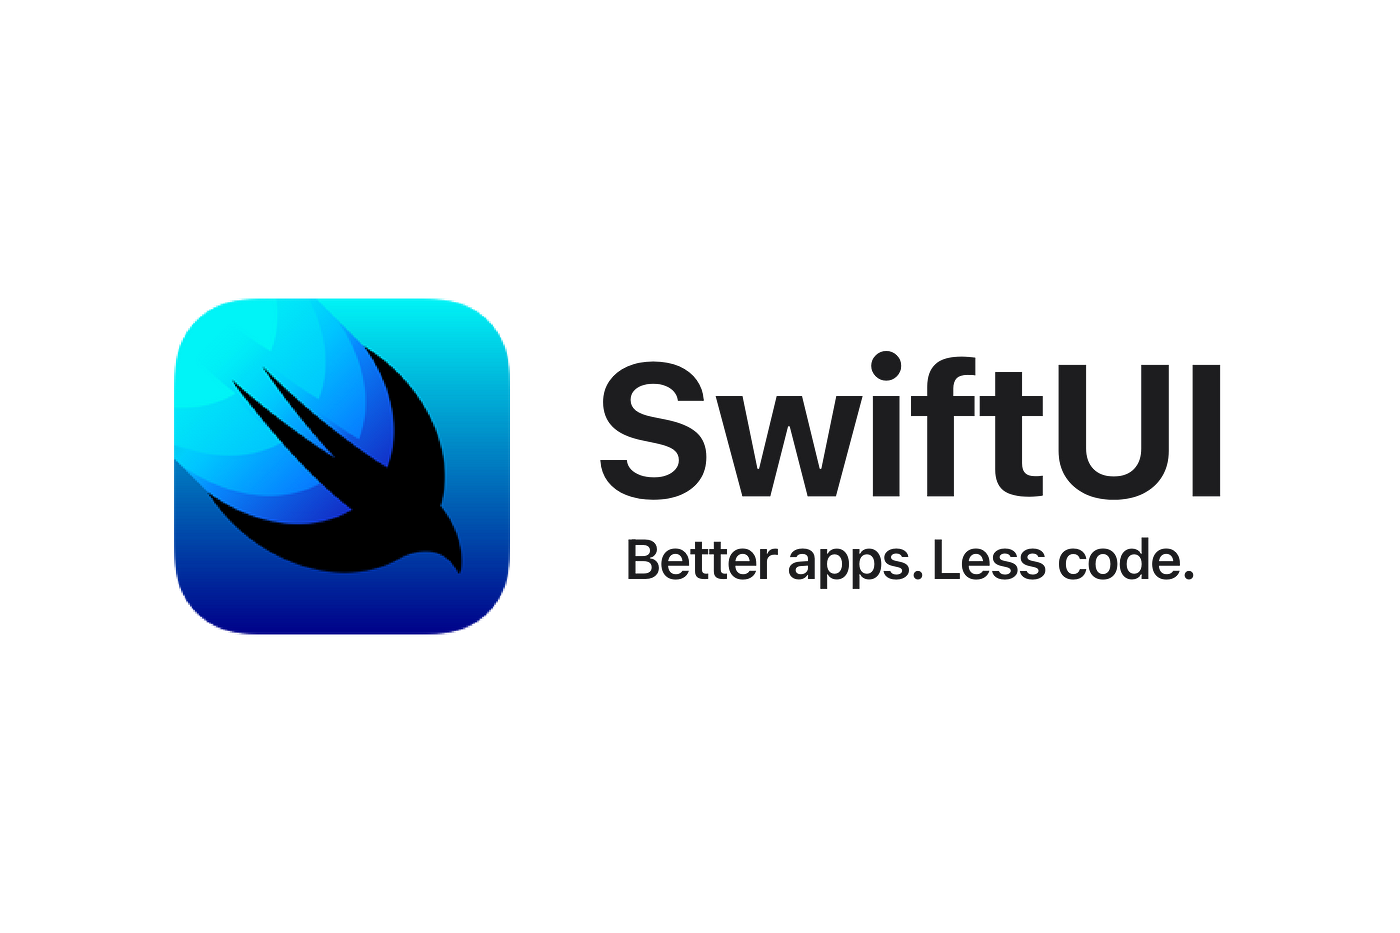
\includegraphics[width=0.3\textwidth]{swiftuibird} 
    \caption{Het swiftUI logo \autocite{SwiftUiImage}}
    \label{fig:swiftUI}
\end{wrapfigure}
Met SwiftUI kun je gebruikersinterfaces bouwen door middel van een reeks van herbruikbare en aanpasbare Views, waardoor je complexe UI-structuren kunt maken met minimale code. Het framework maakt gebruik van een state-driven architectuur, wat betekent dat de UI automatisch wordt bijgewerkt wanneer de toestand van de app verandert. SwiftUI vervangt UIKit als het primaire framework voor het bouwen van interfaces op Apple-platforms, maar het maakt achter de schermen nog steeds vaak gebruik van UIKit-componenten. In deze proef gaan we SwiftUI Views gebruiken om data aan mee te geven om zo performantie te tracken.


\subsection{Views}
\autocite{AppleSwiftViews} Views vormen de bouwstenen van elke SwiftUI-gebruikersinterface. Ze definiëren hoe content wordt weergegeven en gereageerd wordt op gebruikersinteracties. Views kunnen zowel elementaire interface-elementen (zoals tekst, knoppen en afbeeldingen) als complexere composities van deze elementen bevatten.

\begin{figure}[h]
    \begin{minipage}{0.5\textwidth}
        \begin{swift}[caption=Example of a view, label=view_example]
           struct MyView: View {
               var body: some View {
                   Text("Hello, World!")
               }
           }
        \end{swift}
    \end{minipage}%
    \hfill
    \begin{minipage}{0.45\textwidth}
        \centering
        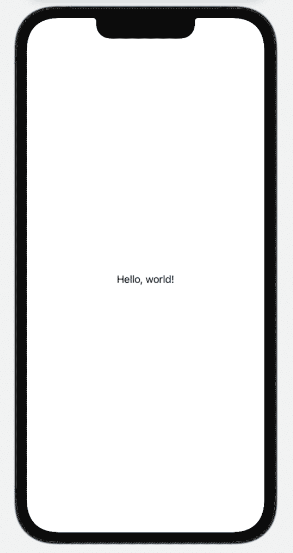
\includegraphics[height=130pt]{helloworldview}
        \caption{Example of a view}
        \label{fig:viewex1}
    \end{minipage}
\end{figure}

\section{Design Patterns}
Design patterns zijn oplossingen voor veelvoorkomende ontwerpproblemen in softwareontwikkeling. Ze bieden gestandaardiseerde en herbruikbare oplossingen voor problemen die zich vaak voordoen tijdens het ontwerpen van software. In Swift met SwiftUI zijn verschillende design patterns van toepassing om de ontwikkeling van robuuste en onderhoudbare apps te vergemakkelijken.

Design Patterns zijn belangerijk voor:
\begin{itemize}
    \item {\textbf{Herbruikbaarheid:} Design patterns bevorderen herbruikbaarheid van code.}
    \item {\textbf{Onderhoudbaarheid:} Ze maken de code gemakkelijker te begrijpen en te onderhouden.}
    \item {\textbf{Schaalbaarheid:} Door het gebruik van design patterns wordt het gemakkelijker om de app uit te breiden en nieuwe functies toe te voegen.}
    \item {\textbf{Testbaarheid:} Code die gebruikmaakt van design patterns is vaak gemakkelijker te testen vanwege de modulaire structuur.}
\end{itemize}
\autocite{MediumPatterns} Enkele belangerijke Design Patterns in Swift met SwiftUI zijn MVVM, MVC, MVP en VIPER.

\subsection{Model-View-ViewModel (MVVM)}
\autocite{MediumMVVM} MVVM is een design pattern dat veel wordt gebruikt in SwiftUI voor het scheiden van de logica van de gebruikersinterface van de onderliggende gegevens. Het bestaat uit drie hoofdcomponenten:
\begin{figure}[H]
    \centering
    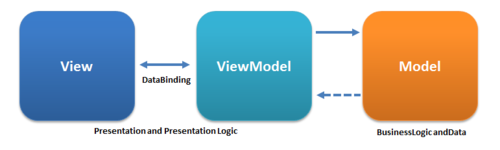
\includegraphics[width=1\textwidth]{MVVMPattern} 
    \caption{MVVM \autocite{MVVMImage}}
    \label{fig:mvvm}
\end{figure}
\begin{itemize}
    \item {\textbf{Model:} Het model bevat de gegevens van de app en de logica voor het manipuleren van die gegevens. Dit is waar de kernfunctionaliteit van de app zich bevindt.}
    \item {\textbf{View:} De view is verantwoordelijk voor het weergeven van de gebruikersinterface en het reageren op gebruikersinteracties. In SwiftUI worden views vaak passief gehouden en bevatten ze minimale logica.}
    \item {\textbf{ViewModel:} De viewmodel fungeert als een tussenliggende laag tussen het model en de view. Het voorziet de view van de gegevens die nodig zijn om te worden weergegeven en reageert op acties van de gebruiker. Het transformeert ook de gegevens van het model naar een vorm die gemakkelijk kan worden weergegeven in de view.}
\end{itemize}
De voordelen van MVVM zijn:
\begin{itemize}
    \item {\textbf{Scheiding van verantwoordelijkheden:} MVVM helpt bij het scheiden van de logica van de gebruikersinterface van de onderliggende gegevens, waardoor de code gemakkelijker te begrijpen en te onderhouden is. Dit zorgt ook voor een eenvoudigere uitbreidbaarheid en herbruikbaarheid van de code.}
    \item {\textbf{Testbaarheid:} Omdat de logica van de gebruikersinterface wordt gescheiden van de gegevenslogica, zijn de componenten gemakkelijker afzonderlijk te testen.}
        \item \textbf{Binding tussen View en ViewModel:} MVVM maakt gebruik van databinding om gegevens tussen de View en de ViewModel te synchroniseren, waardoor de code voor het bijwerken van de gebruikersinterface eenvoudiger en overzichtelijker wordt.
    
    \item \textbf{Flexibiliteit en schaalbaarheid:} Door de scheiding van verantwoordelijkheden kunnen verschillende teams parallel werken aan de ontwikkeling van de gebruikersinterface en de onderliggende gegevenslogica, wat de algehele flexibiliteit en schaalbaarheid van het project ten goede komt.
\end{itemize}

\subsection{VIPER}
\autocite{MediumVIPER} VIPER is een design pattern dat staat voor View, Interactor, Presenter, Entity, en Router. Het is een architectureel patroon dat is ontworpen om de code van een app in verschillende lagen te verdelen om de onderhoudbaarheid en testbaarheid te verbeteren. Hier is een overzicht van de componenten:
\begin{figure}[H]
    \centering
    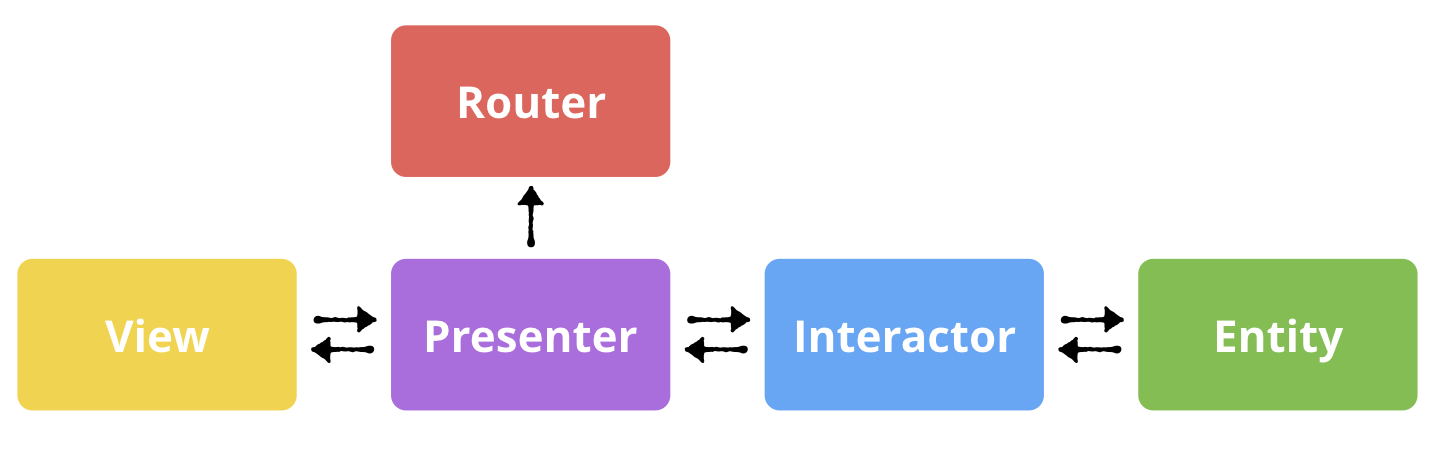
\includegraphics[width=1\textwidth]{viper} 
    \caption{viper \autocite{ViperImage}}
    \label{fig:viper}
\end{figure}

\begin{itemize}
    \item {\textbf{View:} De view is verantwoordelijk voor het weergeven van de gebruikersinterface en het reageren op gebruikersinteracties, vergelijkbaar met MVVM.}
    \item {\textbf{Interactor:} De interactorcomponent bevat de businesslogica van de app. Het is verantwoordelijk voor het ophalen en verwerken van gegevens van externe bronnen, zoals een database of een netwerk.}
    \item {\textbf{Presenter:} De presenter fungeert als een tussenliggende laag tussen de interactor en de view. Het is verantwoordelijk voor het formatteren van de gegevens die zijn verkregen van de interactor en deze door te geven aan de view voor weergave.}
    \item {\textbf{Entity:} De entity bevat de gegevensmodellen van de app. Het vertegenwoordigt de entiteiten die worden gebruikt in de applicatie, zoals gebruikers, items, of andere objecten.}
    \item {\textbf{Router:} De router is verantwoordelijk voor het beheren van de navigatie binnen de app. Het bepaalt welke schermen moeten worden weergegeven en hoe deze moeten worden genavigeerd.}
\end{itemize}
Voordelen van VIPER zijn:
\begin{itemize}
    \item {\textbf{Schaalbaarheid:} Door de code in verschillende lagen te verdelen, maakt VIPER het gemakkelijker om de app uit te breiden en nieuwe functies toe te voegen.}
    \item {\textbf{Testbaarheid:} Elk onderdeel van VIPER kan afzonderlijk worden getest, waardoor het gemakkelijker wordt om bugs op te sporen en te repareren.}
\end{itemize}

\section{XCode Performance Trackers}

In deze proef gericht op het vergelijken van de performantie, rendering en lifescycles van views, zijn Xcode Profiler, Xcode Instruments en XCTest Metrics van onschatbare waarde. Xcode Profiler biedt een basisprofiel van views door CPU-, geheugen- en netwerkactiviteit te meten. Xcode Instruments gaat dieper met gedetailleerde analyses van CPU-, geheugen- en grafische prestaties, en kan rendercycli traceren. XCMetrics biedt automatische verzameling van prestatiegegevens tijdens het uitvoeren van tests. Dit betekent dat tijdens het testen van de code, XCTest Metrics automatisch gegevens verzamelt over de prestaties van de app, waaronder informatie over de tijd die het kost om bepaalde taken uit te voeren, zoals het laden van views. Deze verzamelde gegevens kunnen worden geanalyseerd om prestatieproblemen in de views van de app te identificeren. Het integreren van bevindingen uit deze tools biedt een holistisch beeld van de view-prestaties, waardoor iteratieve optimalisatie mogelijk is voor een verbeterde gebruikerservaring en algehele app-prestaties.



\subsection{Xcode Instruments}
Xcode Instruments is een krachtige tool die wordt geleverd als onderdeel van Apple's Xcode-ontwikkelomgeving. Het stelt ontwikkelaars in staat om diepgaande analyses uit te voeren van de prestaties en het gedrag van hun iOS-, macOS-, watchOS- en tvOS-apps. Met Instruments kunnen ontwikkelaars problemen met prestaties, geheugen, energieverbruik en meer opsporen en diagnosticeren. 

\subsection{XCode Profiler}
Deze tool stelt ontwikkelaars in staat om de prestaties van hun iOS-, macOS-, watchOS- en tvOS-apps te meten en te optimaliseren. De profiler biedt inzicht in de runtime-gedrag van de app, inclusief CPU-gebruik, geheugenverbruik, netwerkactiviteit en meer. Met deze tool kunnen we in deze proef de performantie op basis van CPU-gebruik, geheugenverbruik, enz. gaan meten. 
\paragraph{CPU-profiler}
Hiermee kan men het CPU-gebruik van een app analyseren. Men kan zien welke delen van de code veel CPU-tijd verbruiken en mogelijk optimalisaties doorvoeren om de prestaties te verbeteren.
\begin{figure}[H]
    \centering
    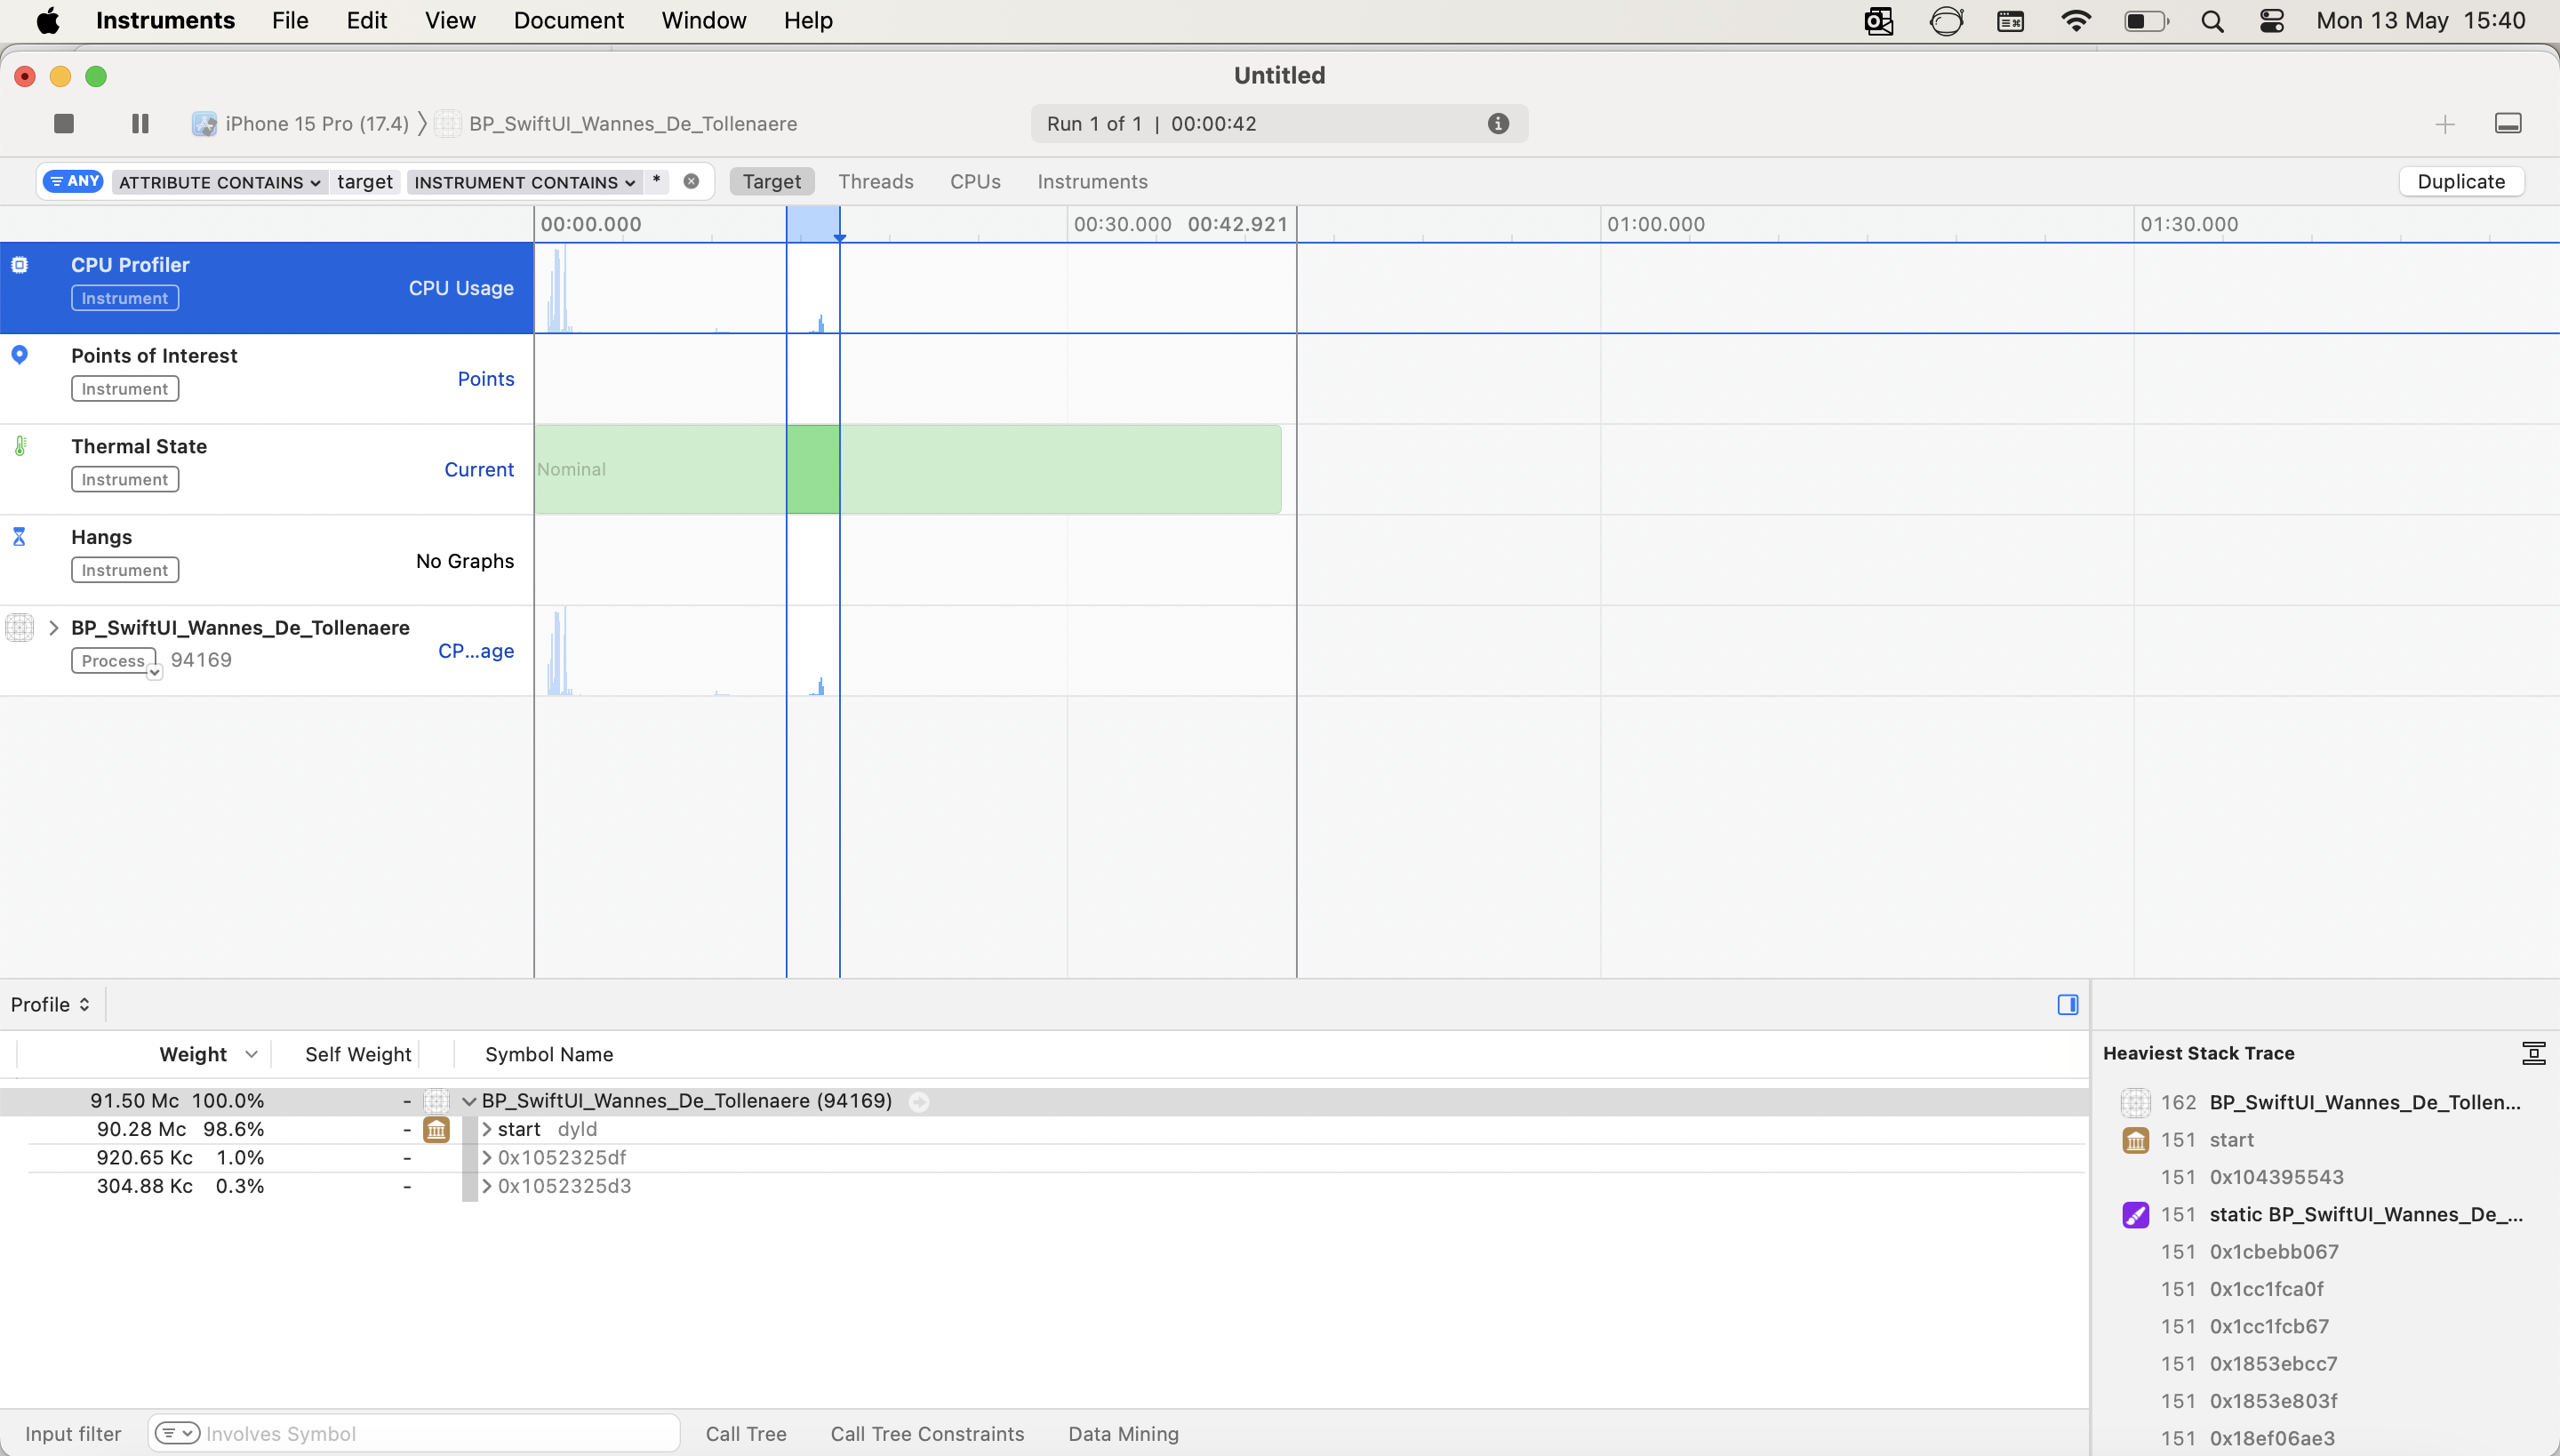
\includegraphics[width=1\textwidth]{BP_XcodeCpuProfiler} 
    \caption{Xcode CPU Profiler}
    \label{fig:cpuProfiler}
\end{figure}
\paragraph{Geheugen-profiler}
Hiermee kan men het geheugenverbruik van een app analyseren. Men kan zien hoeveel geheugen de app gebruikt en hoe dit zich verhoudt tot verschillende delen van de code. Dit kan helpen bij het identificeren van geheugenlekken en het optimaliseren van de geheugenprestaties.
\paragraph{Netwerkprofiler}
Hiermee kan men de netwerkactiviteit van de app analyseren. Men kan zien welke netwerkverzoeken de app maakt en hoe lang deze duren. Dit kan helpen bij het identificeren van trage netwerkverbindingen en het optimaliseren van de netwerkprestaties.

\subsubsection{Realtime monitoring}
Instruments biedt realtime monitoring van de prestaties van een app, waardoor men direct feedback krijgt over het gedrag van een app tijdens het gebruik. Dit stelt ontwikkelaars in staat om problemen snel op te sporen en te diagnosticeren terwijl ze optreden.
\subsubsection{Diepgaande analyse}
Met Instruments kunnen ontwikkelaars diepgaande analyses uitvoeren van de prestaties van hun app. Dit omvat gedetailleerde grafieken, tabellen en visuele hulpmiddelen om inzicht te krijgen in CPU-gebruik, geheugenverbruik, netwerkactiviteit, energieverbruik en meer.
\subsubsection{Tracing en Profiling}
Instruments ondersteunt zowel tracing als profiling van apps. Met tracing kan men het gedrag van een app volgen en analyseren gedurende een bepaalde periode, terwijl profiling men in staat stelt om specifieke aspecten van de prestaties van een app te meten en te optimaliseren.

\subsection{XCTest (Metrics)}
XCTest is een framework dat wordt gebruikt voor het schrijven en uitvoeren van tests in Swift- en Objective-C-gebaseerde applicaties voor iOS, macOS, watchOS en tvOS. Naast de standaard functionaliteit voor het schrijven van tests biedt XCTest ook XCTest Metrics, een functie die ontwikkelaars in staat stelt om verschillende prestatiegerelateerde metingen te verzamelen tijdens het uitvoeren van tests.

\subsubsection{Prestatiemetingen}
XCTest Metrics biedt verschillende metingen voor het evalueren van de prestaties van een app tijdens het uitvoeren van tests. Dit omvat metingen zoals CPU-gebruik, geheugenverbruik, netwerkactiviteit, energieverbruik en meer.
\subsubsection{Ingebouwde instrumenten}
XCTest Metrics maakt gebruik van de ingebouwde Instruments van Xcode om de prestaties van een app te meten. Dit stelt ontwikkelaars in staat om diepgaande analyses uit te voeren van de prestaties van hun app en om potentiële prestatieproblemen te identificeren.
\subsubsection{Grafische Weergave}
XCTest Metrics biedt een grafische weergave van de verzamelde prestatiegegevens, waardoor ontwikkelaars snel inzicht krijgen in de prestaties van hun app tijdens het uitvoeren van tests. Dit omvat grafieken, tabellen en andere visuele hulpmiddelen om trends en patronen te identificeren.
\subsubsection{Automatische Metingen}
XCTest Metrics voert automatisch metingen uit tijdens het uitvoeren van tests, waardoor ontwikkelaars zich kunnen concentreren op het schrijven van tests zonder zich zorgen te hoeven maken over het handmatig meten van prestaties. Dit maakt het gemakkelijker om consistente en betrouwbare metingen te verkrijgen.

\section{SwiftUI View Diffing}

View diffing in SwiftUI is een proces waarbij het framework de huidige staat van de view-hiërarchie vergelijkt met een nieuwe voorgestelde staat en de minimale set wijzigingen berekent die nodig zijn om de UI bij te werken\autocite{ViewDiffing}. Dit proces is cruciaal voor de prestaties, omdat het ervoor zorgt dat alleen de noodzakelijke updates worden uitgevoerd in plaats van de hele view-hiërarchie opnieuw te renderen.

SwiftUI bereikt deze efficiëntie door een combinatie van technieken:

\begin{itemize}
    \item \textbf{Struct-based Views}: SwiftUI views zijn structs, wat waarde types zijn in Swift. Dit betekent dat ze goedkoop zijn om te creëren en te vernietigen, waardoor SwiftUI vrijelijk view-instanties kan maken en weggooien zonder significante overhead.
    \item \textbf{Body Property}: Elke view heeft een \texttt{body}-property die de inhoud definieert. SwiftUI roept deze property aan om de huidige staat van de UI-elementen van de view te krijgen. Als de staat niet is veranderd, wordt de \texttt{body}-property niet opnieuw geëvalueerd, een optimalisatietechniek die bekend staat als memoization.
    \item \textbf{View Identity and State Management}: Door gebruik te maken van unieke sleutels en state management technieken zoals \texttt{@State}, \texttt{@Binding}, en \texttt{@ObservedObject}, kan SwiftUI nauwkeurig bijhouden welke delen van de UI moeten worden bijgewerkt wanneer de onderliggende staat verandert.
\end{itemize}

\section{Combine}
\autocite{AppleCombine} Combine is een declaratief Swift framework dat het mogelijk maakt om reactieve programmeerpatronen te implementeren binnen een applicatie. Het framework is ontworpen om verschillende asynchrone gebeurtenissen te verwerken en te transformeren, waarbij het gebruik maakt van \textit{publishers} en \textit{subscribers} om data te verzenden en te ontvangen. Combine integreert naadloos met Swift en SwiftUI en biedt een consistente manier om data te beheren die afkomstig is van verschillende bronnen, zoals netwerkverzoeken, gebruikersinvoer en nog veel meer. 

Een van de grootste uitdagingen bij de ontwikkeling van moderne applicaties is het beheren van de \textit{state} en het waarborgen van een soepele en consistente dataoverdracht tussen verschillende onderdelen van de UI. Combine biedt een robuuste oplossing voor deze uitdaging door middel van zijn reactieve programmeermodel, wat directe implicaties heeft voor de manier waarop \textit{views} met elkaar communiceren en data delen.

\section{Annotations}
\subsection{@propertyWrapper}
\autocite{ApplePropertyWrapper} Property wrappers in Swift fungeren als een tussenlaag tussen de eigenschap zelf en de code die de opslag, verwerking of transformatie van de waarde van die eigenschap beheert. Deze abstractielaag biedt een gestructureerde manier om het gedrag van eigenschappen te definiëren en te beheren, waardoor de leesbaarheid, herbruikbaarheid en onderhoudbaarheid van de code worden verbeterd.

Ze kunnen worden toegepast op zowel opgeslagen als berekende eigenschappen en stellen ontwikkelaars in staat om complexe logica te isoleren die nodig is voor het beheer van een eigenschap. Door het gebruik van property wrappers kunnen ontwikkelaars specifieke gedragingen voor eigenschappen definiëren, zoals validatie van waarden, lazy loading, caching en toegangscontrole.

Property wrappers zijn een krachtige tool in Swift, omdat ze een compacte en elegante manier bieden om het gedrag van eigenschappen aan te passen en complexe logica te abstraheren, wat resulteert in een consistente en duidelijke codebase.
\begin{swift}[caption=Example property wrapper code \autocite{PropertyWrapperExample}, label=property_wrapper_example]
    @propertyWrapper
    struct TwelveOrLess {
        private var number = 0
        var wrappedValue: Int {
            get { return number }
            set { number = min(newValue, 12) }
        }
    }
    
    struct SmallRectangle {
        @TwelveOrLess var height: Int
        @TwelveOrLess var width: Int
    }
    
    
    var rectangle = SmallRectangle()
    print(rectangle.height)
    // Prints "0"
    
    
    rectangle.height = 10
    print(rectangle.height)
    // Prints "10"
    
    
    rectangle.height = 24
    print(rectangle.height)
    // Prints "12"
\end{swift}


\subsection{@State}
\autocite{AppleState} State is een property wrapper die een waarde kan lezen en schrijven die wordt beheerd door SwiftUI. Het wordt gebruikt als de enige bron van de 'waarheid' (truth) voor een gegeven value type die binnen de view hierarchy wordt opgeslagen. State wordt gebruikt voor het beheren van lokale toestanden binnen een view, waarbij het automatisch reageren op wijzigingen in de waarde en het opnieuw renderen van de bijbehorende view.

\begin{swift}[caption=Example of @State code \autocite{AppleState}, label=state_example]
    struct PlayButton: View {
        @State private var isPlaying: Bool = false // Create the state.
        
        
        var body: some View {
            Button(isPlaying ? "Pause" : "Play") { // Read the state.
                isPlaying.toggle() // Write the state.
            }
        }
    }
\end{swift}


\subsection{@Binding}
\autocite{AppleBinding} Binding wordt gebruikt om een tweewegsverbinding tot stand te brengen tussen een eigenschap die gegevens opslaat en een weergave die de gegevens presenteert. Een binding verbindt een eigenschap met een bron van "truth" (waarheid), wat betekent dat het niet zelf de gegevens opslaat, maar eerder verwijst naar de bron waar de gegevens worden bewaard. Dit maakt het mogelijk dat wijzigingen in de bron onmiddellijk worden weerspiegeld in de weergave, en omgekeerd. Bijvoorbeeld, als de waarde van de eigenschap wordt gewijzigd, wordt de bijbehorende weergave automatisch bijgewerkt om de nieuwe waarde weer te geven. En als de gebruiker de waarde in de weergave wijzigt, worden de gegevens in de bron automatisch bijgewerkt om deze wijzigingen weer te geven.

\begin{swift}[caption=Example of @Binding code \autocite{AppleBinding}, label=binding_example]
    struct PlayButton: View {
        @Binding var isPlaying: Bool
        
        
        var body: some View {
            Button(isPlaying ? "Pause" : "Play") {
                isPlaying.toggle()
            }
        }
    }
    
    struct PlayerView: View {
        var episode: Episode
        @State private var isPlaying: Bool = false
        
        
        var body: some View {
            VStack {
                Text(episode.title)
                .foregroundStyle(isPlaying ? .primary : .secondary)
                PlayButton(isPlaying: $isPlaying) // Pass a binding.
            }
        }
    }
\end{swift}


\subsection{@ObservableObject}
\autocite{AppleObservableObject} Een ObservableObject is een object dat in staat is veranderingen in zijn staat te detecteren en hier melding van te maken aan geïnteresseerde partijen, via het Observer-patroon. Dit concept is van cruciaal belang bij het ontwikkelen van applicaties met een reactieve programmeerstijl. Wanneer een ObservableObject wordt gewijzigd, stuurt het automatisch een signaal (meestal objectWillChange) naar alle geabonneerde views of componenten, waardoor ze op de hoogte worden gebracht van de verandering. Dit stelt de views in staat om hun weergave bijgevolg bij te werken, wat zorgt voor een dynamische en reactieve gebruikerservaring. Bijvoorbeeld, een view kan zich abonneren op veranderingen in een ObservableObject en automatisch worden bijgewerkt wanneer de staat van dat object verandert.

\subsubsection{Observer Pattern}
\autocite{MediumDesignPatterns} Dit patroon is een gedragspatroon waarbij een object, dat de 'observable' of 'subject' wordt genoemd, een lijst met afhankelijkheden bijhoudt, ook wel 'observers' genoemd. Wanneer het observable object verandert, worden alle geïnteresseerde observers op de hoogte gesteld van deze verandering.

\subsubsection{@Published}
\autocite{ApplePublished} De eenvoudigste manier om een object als observable te maken, is door de @Published-property wrapper te gebruiken voor eigenschappen die je wilt observeren. Wanneer de waarde van een eigenschap die is gemarkeerd met @Published verandert, zal het observable object automatisch melding maken van deze verandering aan alle geabonneerde observers.

\begin{swift}[caption=Example of implemented Observable Pattern \autocite{AppleObservableObject}, label=observable_example]
class Contact: ObservableObject {
    @Published var name: String
    @Published var age: Int
    
    
    init(name: String, age: Int) {
        self.name = name
        self.age = age
    }
    
    
    func haveBirthday() -> Int {
        age += 1
        return age
    }
}


let john = Contact(name: "John Appleseed", age: 24)
cancellable = john.objectWillChange
.sink { _ in
    print("(john.age) will change")
}
print(john.haveBirthday())
// Prints "24 will change"
// Prints "25"
\end{swift}

\subsection{@StateObject}
\Autocite{AppleStateObject} StateObject is een property wrapper in SwiftUI, waarmee je een instantie van een observable object kunt maken en behouden gedurende de levensduur van een specifieke SwiftUI View. Dit is handig wanneer je een observable object wilt gebruiken om de staat van een weergave te beheren, maar je wilt niet dat deze wordt gedeeld tussen verschillende instanties van dezelfde weergave.

\begin{swift}[caption=Example of StateObject, label=stateobject_example]
class MyData: ObservableObject {
    @Published var value: Int = 0
}

struct ContentView: View {
    @StateObject var data = MyData()
    
    var body: some View {
        VStack {
            ChildView(data: data)
            AnotherChildView(data: data)
        }
    }
}

struct ChildView: View {
    @ObservedObject var data: MyData
    
    var body: some View {
        VStack {
            Text("Value in ChildView: (data.value)")
            Button("Increment in ChildView") {
                data.value += 1
            }
        }
    }
}
struct AnotherChildView: View {
    @ObservedObject var data: MyData
    
    var body: some View {
        VStack {
            Text("Value in AnotherChildView: (data.value)")
            Button("Increment in AnotherChildView") {
                data.value += 1
            }
        }
    }
}

\end{swift}

\subsection{Verschil @StateObject en @ObservedObject}
\autocite{MediumDifferenceStateObjObservedObj} @StateObject en @ObservedObject hebben gelijkaardige functies, maar verschillen in hoe SwiftUI hun levenscyclus beheert. Met @StateObject wordt het waargenomen object automatisch geïnitialiseerd en behouden door SwiftUI, wat consistentie garandeert wanneer de huidige weergave het waargenomen object creëert. Dit kan een positieve invloed hebben op het CPU-gebruik, omdat het efficiënter is wanneer SwiftUI direct de levenscyclus van het object beheert. Aan de andere kant wordt @ObservedObject gebruikt wanneer een waargenomen object wordt geïnjecteerd als een afhankelijkheid, waarbij SwiftUI veranderingen in het object detecteert en de weergave bijwerkt.

\subsection{@Observable}
\autocite{AppleObservable}, \autocite{ObservablePerformance} Het gebruik van @Observable in SwiftUI helpt onnodige Swift redraws te vermijden. Deze macro, beschikbaar vanaf iOS 17.0 en later, dient als een essentieel instrument voor het implementeren van het observer-patroon. Het vervangt eerdere macro's die voor dit doel werden gebruikt en biedt ontwikkelaars een eenvoudige manier om eigenschappen te markeren die veranderingen moeten doorgeven aan views of andere componenten die geïnteresseerd zijn in die veranderingen. Wanneer een eigenschap die is geannoteerd met @Observable wordt gewijzigd, wordt automatisch een signaal verzonden naar alle views die eraan zijn gekoppeld, waardoor ze hun weergave dienovereenkomstig kunnen bijwerken. Dit biedt een krachtige en efficiënte manier om reactieve gebruikersinterfaces te bouwen in SwiftUI.

\begin{swift}[caption=Example of Observable, label=Observable_example]
// ViewModel met @Observable macro
@Observable class SimpleViewModel {
    var text = "Hello World :)"
}

// SwiftUI View
struct SimpleView: View {
    @Environment(SimpleViewModel.self) var viewModel
    
    var body: some View {
        Text(viewModel.text)
    }
}
\end{swift}


\subsection{@Environment}
\autocite{AppleEnvironment} In SwiftUI biedt @Environment een mechanisme om waarden door te geven door de view-hiërarchie, zonder ze expliciet door te geven aan elke view als afzonderlijke eigenschappen. Het maakt gebruik van de omgeving van de View om gegevens te delen tussen Views in een hiërarchie. Dit is handig voor het doorgeven van gegevens die van toepassing zijn op de hele app of een deel ervan, zoals thema's, kleuren, taalinstellingen, enzovoort. Met @Environment kunnen views eenvoudig toegang krijgen tot deze gedeelde gegevens zonder dat ze expliciet aan elke view hoeven te worden doorgegeven, waardoor de code schoner en gemakkelijker te onderhouden wordt. Bijvoorbeeld, als de app een bepaald thema heeft ingesteld, kunnen alle views binnen de hiërarchie eenvoudig toegang krijgen tot het thema met behulp van @Environment, zonder dat het thema expliciet aan elke view hoeft te worden doorgegeven. Dit verbetert de modulariteit en flexibiliteit van de codebase.


\begin{swift}[caption=Example of Environment, label=Environment_example]
struct ContentView: View {
    @Environment(\.colorScheme) var colorScheme
    
    var body: some View {
        VStack {
            Text("Current color scheme is (colorScheme)")
            ChildView()
        }
    }
}

struct ChildView: View {
    var body: some View {
        Text("This is a child view")
    }
}
\end{swift}

\subsection{@EnvironmentObject}
\autocite{AppleEnvironmentObject} @EnvironmentObject in SwiftUI biedt een handig mechanisme om gedeelde gegevens door te geven aan views in de view-hiërarchie. Het maakt het mogelijk om een ObservableObject te registreren op het hoogste niveau van de app, waardoor het automatisch beschikbaar wordt gesteld aan alle onderliggende views. Hierdoor kunnen views gemakkelijk toegang krijgen tot deze gedeelde gegevens zonder dat ze expliciet aan elke view moeten worden doorgegeven. Dit bevordert een efficiënte en nette manier om gedeelde staat binnen een SwiftUI-app te beheren.


\begin{swift}[caption=Example of EnvironmentObject, label=EnvironmentObject_example]
    class SharedData: ObservableObject {
        @Published var text = "Hallo, wereld!"
    }
    
    struct ContentView: View {
        @EnvironmentObject var sharedData: SharedData
        
        var body: some View {
            Text(sharedData.text)
        }
    }

    struct MyView: View {
        @StateObject var sharedData = SharedData()
        
        var body: some View {
            ContentView().environmentObject(sharedData)
        }
    }
\end{swift}


%%=============================================================================
%% Methodologie
%%=============================================================================

\chapter{\IfLanguageName{dutch}{Methodologie}{Methodology}}%
\label{ch:methodologie}

%% TODO: In dit hoofstuk geef je een korte toelichting over hoe je te werk bent
%% gegaan. Verdeel je onderzoek in grote fasen, en licht in elke fase toe wat
%% de doelstelling was, welke deliverables daar uit gekomen zijn, en welke
%% onderzoeksmethoden je daarbij toegepast hebt. Verantwoord waarom je
%% op deze manier te werk gegaan bent.
%% 
%% Voorbeelden van zulke fasen zijn: literatuurstudie, opstellen van een
%% requirements-analyse, opstellen long-list (bij vergelijkende studie),
%% selectie van geschikte tools (bij vergelijkende studie, "short-list"),
%% opzetten testopstelling/PoC, uitvoeren testen en verzamelen
%% van resultaten, analyse van resultaten, ...
%%
%% !!!!! LET OP !!!!!
%%
%% Het is uitdrukkelijk NIET de bedoeling dat je het grootste deel van de corpus
%% van je bachelorproef in dit hoofstuk verwerkt! Dit hoofdstuk is eerder een
%% kort overzicht van je plan van aanpak.
%%
%% Maak voor elke fase (behalve het literatuuronderzoek) een NIEUW HOOFDSTUK aan
%% en geef het een gepaste titel.
\section{long-list}
\subsection{dataoverdrachtsmethoden}
Deze opties bieden verschillende benaderingen om gegevens door te geven aan SwiftUI-views.
\begin{itemize}
    \item {\textbf{State properties:} In SwiftUI kunnen gegevens door middel van @State-eigenschappen aan views worden doorgegeven. Deze optie omvat verschillende manieren waarop state-eigenschappen kunnen worden gebruikt om views dynamisch te updaten.}
    \item {\textbf{Binding properties:} @Binding-eigenschappen bieden een manier om gegevens tussen een parent view en een child view te synchroniseren, zodat wijzigingen in een child view ook de parent view beïnvloeden.}
    \item {\textbf{Observed objects:} Met @ObservedObject kunnen views gegevens volgen van een modelobject dat conform ObservableObject is. Dit maakt het mogelijk om complexere data-infrastructuren op te bouwen.}
    \item {\textbf{Environment objects:} @EnvironmentObject maakt het mogelijk om een object door te geven aan verschillende views in de SwiftUI-hiërarchie, zodat dezelfde gegevens gedeeld kunnen worden zonder dat ze expliciet door elke view moeten worden doorgegeven.}s
    \item {\textbf{State objects:} @StateObject is een eigenschap die wordt gebruikt om de levensduur van een object dat conform ObservableObject is, in een SwiftUI-view te beheren. Dit wordt vaak gebruikt om een modelobject te creëren dat het hele leven van de view meegaat.}
    \item {\textbf{View models:} Een view model wordt vaak gebruikt in de Model-View-ViewModel (MVVM) architectuur. Deze optie omvat het gebruik van een view model om gegevens en logica te beheren, en deze vervolgens aan de SwiftUI-views door te geven.}
    \item {\textbf{Data publishers:} In SwiftUI kunnen Combine-publishers worden gebruikt om gegevensstromen te beheren en automatisch aan views door te geven. Dit maakt het mogelijk om data-reactief gedrag te implementeren, waarbij views automatisch worden bijgewerkt wanneer de gegevens wijzigen.}
\end{itemize}
\subsection{testtools}
Deze lijst biedt verschillende testtools die kunnen worden gebruikt om SwiftUI-applicaties te testen en te profileren.
\begin{itemize}
    \item {\textbf{Xcode Profiler:} Xcode bevat ingebouwde profileringsinstrumenten waarmee je de prestaties van je applicatie kunt analyseren, zoals CPU- en geheugengebruik. Je kunt specifieke gebieden van je code profileren en optimalisaties uitvoeren om de efficiëntie te verbeteren.}
    \item {\textbf{XCTest:} XCTest is de standaard testframework in Xcode en wordt gebruikt voor het schrijven van eenheidstests en UI-tests voor SwiftUI-applicaties. Je kunt hiermee testcases definiëren en asserties uitvoeren om de correctheid van je code te waarborgen.}
    \item {\textbf{Instruments:} Instruments is een uitgebreide set van profilerings- en monitoringtools die beschikbaar zijn in Xcode. Je kunt hiermee verschillende aspecten van je applicatie analyseren, zoals netwerkverkeer, batterijverbruik, en geheugenlekken.}
    \item {\textbf{AppCode:} AppCode is een IDE voor iOS-ontwikkeling die ondersteuning biedt voor het schrijven en uitvoeren van tests in SwiftUI-applicaties. Het bevat ook tools voor code-analyse, debugging, en profilering.}
    \item {\textbf{View Inspector:} View Inspector is een tool waarmee je de compositie van SwiftUI-views kunt analyseren en inspecteren. Dit kan nuttig zijn voor het debuggen van complexe view-hiërarchieën.}
    \item {\textbf{KIF (Keep It Functional):} KIF is een testframework waarmee je functionele tests kunt schrijven voor iOS-applicaties, inclusief SwiftUI-applicaties. Het stelt je in staat om tests te schrijven in een leesbare, natuurlijke taal.}
    \item {\textbf{Snapshot testing:} Snapshot testing is een techniek waarbij je de weergave van een view opslaat en vergelijkt met een eerdere "snapshot" om te controleren of de weergave ongewijzigd is gebleven. Er zijn verschillende tools beschikbaar voor het uitvoeren van snapshot-tests in SwiftUI, zoals SnapshotTesting.}
    \item {\textbf{Quick and Nimble:} Quick is een testframework dat gericht is op het schrijven van gestructureerde en leesbare tests. Nimble is een bijbehorende assertiebibliotheek die expressieve asserties biedt om testcases eenvoudiger te maken.}
\end{itemize}
\section{testopstelling}
Een testomgeving is gecreëerd door SwiftUI-views te ontwikkelen voor elke methode van dataoverdracht. Elke view heeft een groot databestand ontvangen, dat binnen de view is aangepast om nieuwe rendercyclussen te activeren. Dit proces is herhaald voor elke overdrachtsmethode en het gemiddelde geheugengebruik, CPU-gebruik en laadtijd van deze views is berekend. Deze gegevens zijn waargenomen met behulp van de eerder genoemde tools. Door de verzamelde gegevens te vergelijken, is een conclusie getrokken over de meest efficiënte methode. 

\section{analyse van resultaten}
Tijdens de proef zijn gegevens verzameld over het aantal keren dat SwiftUI-views werden ververst tijdens dataoverdracht en de prestaties van verschillende overdrachtsmethoden. Deze resultaten zijn geanalyseerd om inzicht te krijgen in de efficiëntie en impact van elke methode op de applicatie.

Het gemiddelde geheugengebruik, CPU-gebruik en de laadtijd van de views zijn berekend voor elke methode van dataoverdracht. De analyse van deze gegevens heeft geholpen om patronen en trends in de prestaties van de verschillende methoden te identificeren. Daarnaast zijn de frequentie en duur van rendercyclussen onderzocht om mogelijke knelpunten in de code te achterhalen.

Op basis van deze analyse zijn aanbevelingen gedaan voor de meest efficiënte dataoverdrachtsmethoden voor SwiftUI-views. Dit biedt waardevolle inzichten voor de optimalisatie van SwiftUI-applicaties en het verbeteren van de algehele gebruikerservaring. De resultaten vormen de basis voor verdere ontwikkeling en optimalisatie van SwiftUI-applicaties in toekomstige projecten.



% Voeg hier je eigen hoofdstukken toe die de ``corpus'' van je bachelorproef
% vormen. De structuur en titels hangen af van je eigen onderzoek. Je kan bv.
% elke fase in je onderzoek in een apart hoofdstuk bespreken.

%\input{...}
%\input{...}
%...
\chapter{Ruwe resultaten}%
\label{ch:ruweresultaten}
In dit deel word er over alle ruwe resultaten gegaan. Elke afbeelding in dit hoofdstuk bevatten rechtstreekse resultaten vanuit de XCode Profiler. Bij deze afbeeldingen word er ook een kort woordje uitleg gedaan die de resultaten beschrijven.

Voor het meten van het CPU verbruik tijdens het testen van verschillende methoden van data-overdracht is de Xcode profiling tool gebruikt met als template de CPU profiler. Met deze tool is gemeten hoeveel Mc(Mega cycles, cycle = 
de tijd die nodig is voor de uitvoering van één eenvoudige processorbewerking) de app vereist heeft van de CPU per type van data-overdracht. 

Voor het meten van het aantal updates van verschillende view property's, view refreshes en totale CPU gebruik tijd tijdens het testen van verschillende methoden van data-overdracht is de Xcode profiling tool gebruikt met als template de Swift-UI profiler. 

\section{test1: het testen op een lege view met grote dataoverdracht}
\subsection{CPU verbruik}

\paragraph{binding}
Uit de tabel blijkt dat wanneer we een binding gebruiken om een groot object door te geven aan een view, en we maken een aanpassing in die view, dit ongeveer 14,08 mega cycli van de CPU vereist. Bindings worden voornamelijk voor primitieve types gebruikt, maar voor dit onderzoek word er een groot object aan meegegeven.
\begin{figure}[H]
    \centering
    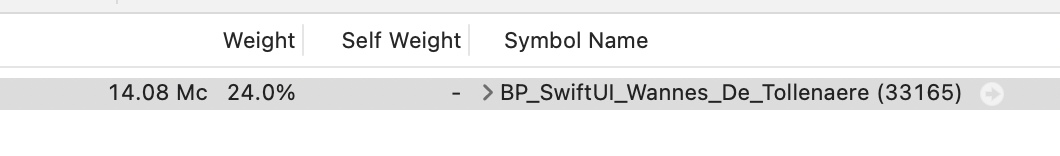
\includegraphics[width=1\textwidth]{BP_CpuUsageBinding} 
    \caption{test1: CPU gebruik van binding}
    \label{fig:cpuBinding}
\end{figure}

\paragraph{environment}
Uit de tabel blijkt dat het gebruik van Environment om een groot object door te geven aan een view, en het vervolgens aanpassen van dat object, ongeveer 250,08 kilocycli van de CPU vereist.
\begin{figure}[H]
    \centering
    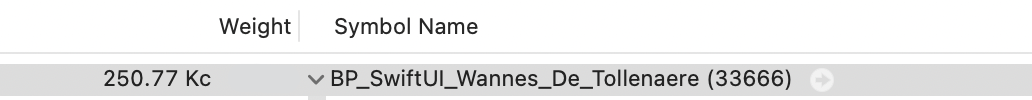
\includegraphics[width=1\textwidth]{BP_CpuUsageEnvironment} 
    \caption{test1: CPU gebruik van environment}
    \label{fig:cpuEnvironment}
\end{figure}

\paragraph{environmentObject}
Uit de tabel blijkt dat het gebruik van een environmentObject om een groot object door te geven aan een view, en het vervolgens aanpassen van dat object, ongeveer 17,13 mega cycli van de CPU vereist.
\begin{figure}[H]
    \centering
    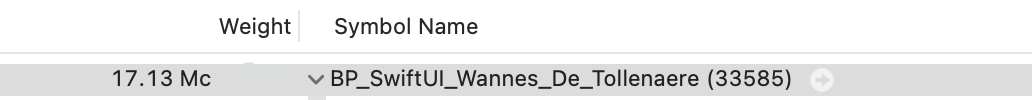
\includegraphics[width=1\textwidth]{BP_CpuUsageEnvironmentObject} 
    \caption{test1: CPU gebruik van environmentObject}
    \label{fig:cpuEnvironmentObject}
\end{figure}

\paragraph{observable}
Uit de tabel blijkt dat wanneer we een Observable gebruiken om een groot object door te geven aan een view, en we vervolgens een aanpassing aan dat object in die view maken, dit ongeveer 19,45 mega cycli van de CPU vereist.
\begin{figure}[H]
    \centering
    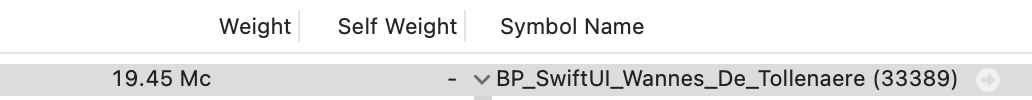
\includegraphics[width=1\textwidth]{BP_CpuUsageObservable} 
    \caption{test1: CPU gebruik van een Observable}
    \label{fig:cpuObservable}
\end{figure}\

\paragraph{observableObject}
Uit de tabel blijkt dat wanneer we een observableObject gebruiken om een groot object door te geven aan een view, en we vervolgens een aanpassing aan dat object in die view maken, dit ongeveer 17,82 mega cycli van de CPU vereist.
\begin{figure}[H]
    \centering
    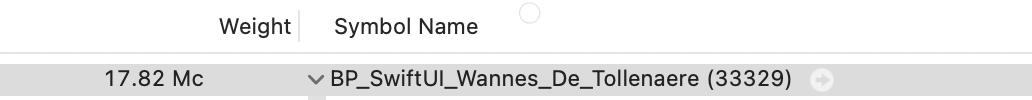
\includegraphics[width=1\textwidth]{BP_CpuUsageObservedObject} 
    \caption{test1: CPU gebruik van observableObject}
    \label{fig:cpuObservedObject}
\end{figure}

\paragraph{without property wrappers}
Uit de tabel blijkt dat het simpelweg doorgeven van een groot object aan een view zonder speciale annotaties, en zonder er vervolgens aanpassingen op te maken, gemiddeld 2,00 mega cycli van de CPU verbruikt.
\begin{figure}[H]
    \centering
    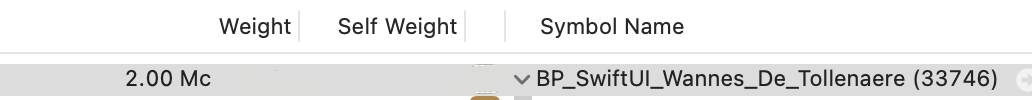
\includegraphics[width=1\textwidth]{BP_CpuUsageWithoutPropertyWrapper} 
    \caption{test1: CPU gebruik van een view zonder property wrappers}
    \label{fig:cpuWithoutPropertyWrapper}
\end{figure}

\newpage
\subsection{Property updates}
\paragraph{Snellere reactiesnelheid}
Binding, ObservedObject en EnvironmentObject passen de property bij elke wijziging tweemaal aan, wat zorgt voor een snellere en consistenter bijgewerkte state. Deze methoden zijn geschikt voor applicaties waarbij real-time gegevensuitwisseling en een directe reactie op veranderingen essentieel zijn, zoals een chatapplicatie of een live-dashboard.

\paragraph{Tragere reactiesnelheid}
Daarentegen voeren Observable en Environment slechts één update per aanpassing uit, wat kan resulteren in minder efficiënte of langzamere reacties op veranderingen. Deze methoden kunnen beter geschikt zijn voor applicaties waar updates minder frequent zijn of waar de responsietijd minder kritisch is, zoals een notitie-app of een takenbeheer-app.


\begin{figure}[H]
    \centering
    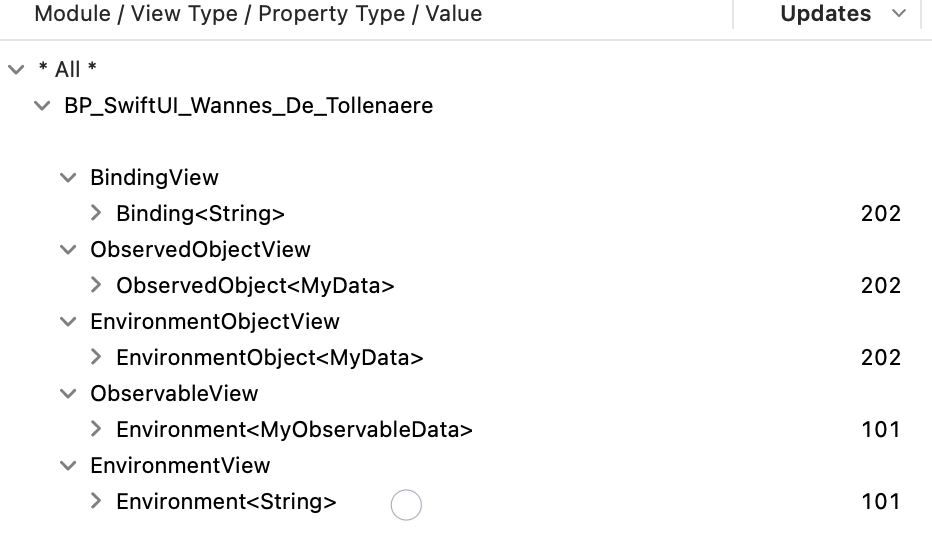
\includegraphics[width=1\textwidth]{BP_ViewPropertyUpdates} 
    \caption{test1: Aantal keren dat de property's geupdate zijn bij het 101 keer opnieuw toewijzen}
    \label{fig:propertyUpdates}
\end{figure}

\newpage
\subsection{View refresh time}
Voor het meten van het gemiddelde view refresh times van SwiftUI Views tijdens het testen van verschillende methoden van data-overdracht is de Xcode profiling tool gebruikt met als template de SwiftUI profiler. De resultaten zijn waargenomen door een view aan te maken, de data door te geven volgens de methode die aangegeven is. Vervolgens de data updaten. Dit 100x herhalen voor elk type View. Ten slotte de gemiddelde tijdswaarden aflezen in de Xcode profiler.

\begin{figure}[H]
    \centering
    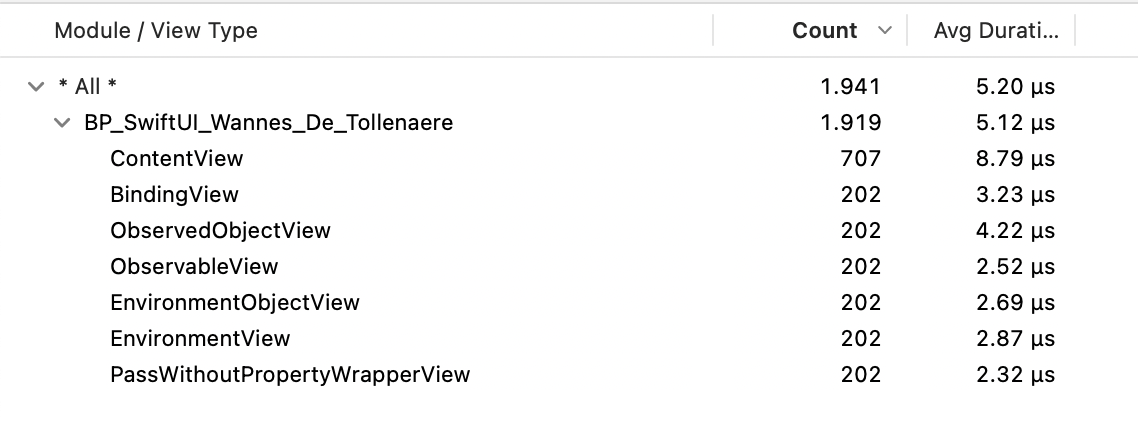
\includegraphics[width=1\textwidth]{BP_ViewRefreshCountAvgDuration} 
    \caption{test1: Gemiddelde duratie voor de view om in te laden per property type}
    \label{fig:propertyRefreshDuration}
\end{figure}

\section{test2: Dataoverdracht in subview's}
In deze sectie word de applicatie in de afbeelding hieronder gebruikt om de testen uit te voeren. Opgebouwd uit 1 VStack's die 10 HStack's bevat per HStack worden er 10 Tegels weergegeven. Elke tegel is zeer CPU heavy opgebouwd zodat de resultaten meer zichtbaar worden in de testen. Elke tile bevat ook een knop die een aanpassing van de testbare data gaat triggeren. In volgende afbeelding word de hierarchy afgebeeld. Voor elk type van dataoverdracht is er 10 keer op de button gedrukt voor het wijzigen van de view. Zo zijn de metingen tot stand gekomen. Alle ruwe resultaten die waargenomen zijn per datatype kan u terugvinden in bijlagen onder sectie test2: Dataoverdracht in subview's. 
\begin{figure}[H]
    \centering
    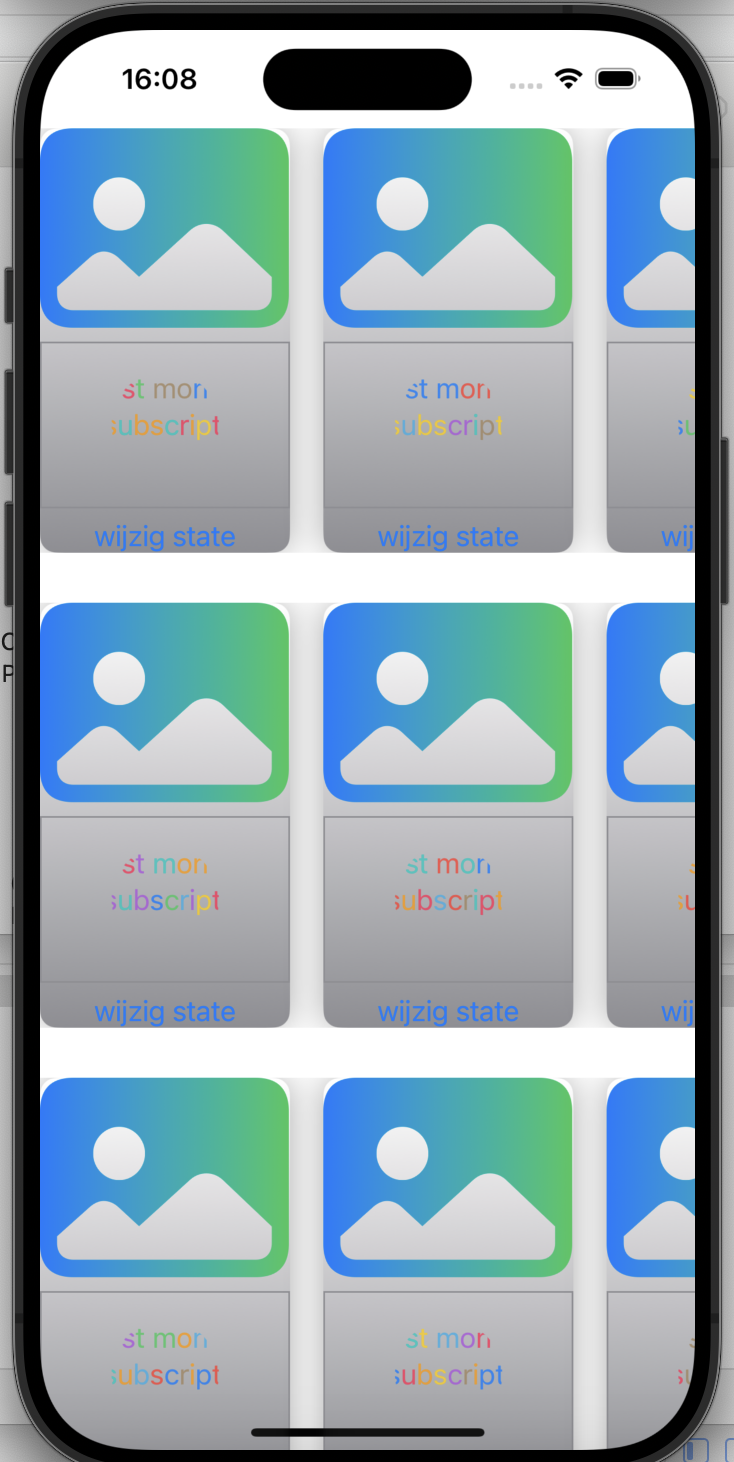
\includegraphics[width=0.4\textwidth]{testapplication} 
    \caption{testapplicatie}
    \label{fig:testapplication}
\end{figure}
\begin{figure}[H]
    \centering
    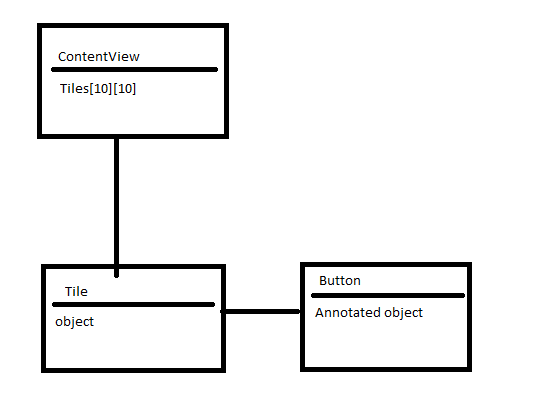
\includegraphics[width=0.4\textwidth]{bptest1_insubview/dataHierarchy} 
    \caption{testapplicatie data hierarchy}
    \label{fig:testapplicationHierarchy}
\end{figure}

\subsection{Samengevat}
Onderstaande tabel bevat alle samengevatte resultaten uit deze test in 1 tabel gegoten. Uit deze tabel word er later in deze proef een conclusie getrokken.
\newpage
\begin{table}[H]
    \centering
    \begin{tabularx}{\textwidth}{|>{\raggedright\arraybackslash}m{5cm}|X|X|X|X|}
        \hline
        \textbf{Description} & \textbf{Binding} & \textbf{Observable} & \textbf{Environment Object} & \textbf{Observable Object} \\
        \hline
        \multicolumn{5}{|l|}{\textbf{Refresh count}} \\
        \hline
        ContentView refresh count & 0 & 0 & 0 & 0 \\
        \hline
        TileView refresh count & 10 & 10 & 0 & 0 \\
        \hline
        Button refresh count & 10 & 0 & 10 & 10 \\
        \hline
        Total refresh count & 20 & 10 & 10 & 10 \\
        \hline
        \multicolumn{5}{|l|}{\textbf{Refresh duration}} \\
        \hline
        ContentView total refresh duration & N.V.T & N.V.T & N.V.T & N.V.T \\
        \hline
        TileView total refresh duration & 393,62 \textmu s & 1,82 ms & N.V.T & N.V.T \\
        \hline
        Button total refresh duration & 104,46 \textmu s & N.V.T & 214,58 \textmu s & 125,63 \textmu s \\
        \hline
        Total duration & 498,08 \textmu s & 1,82 ms & 214,58 \textmu s & 125,63 \textmu s \\
        \hline
        ContentView average refresh duration & N.V.T & N.V.T & N.V.T & N.V.T \\
        \hline
        TileView average refresh duration & 39,36 \textmu s & 181,93 \textmu s & N.V.T & N.V.T \\
        \hline
        Button average refresh duration & 10,45 \textmu s & N.V.T & 21,56 \textmu s & 12,56 \textmu s \\
        \hline
        \multicolumn{5}{|l|}{\textbf{View property updates}} \\
        \hline
        ContentView property updates & N.V.T & N.V.T & N.V.T & N.V.T \\
        \hline
        TileView property updates & 10 & 10 & 0 & 0 \\
        \hline
        Button property updates & 10 & 0 & 10 & 10 \\
        \hline
        Total property updates & 20 & 10 & 10 & 10 \\
        \hline
        \multicolumn{5}{|l|}{\textbf{CPU usage}} \\
        \hline
        Total CPU usage time & 481 ms & 400 ms & 401 ms & 447 ms \\
        \hline
        Total CPU weight & 245,72 Mc & 294,88 Mc & 243,61 Mc & 653,23 Mc \\
        \hline
    \end{tabularx}
    \caption{Performance metrics comparison}
    \label{tab:performance_metrics}
\end{table}


\section{Test3: Dataoverdracht naar meerdere subview's met lazyLists}
% Binding test 2
In deze sectie word de applicatie in de afbeelding hieronder gebruikt om de testen uit te voeren. Opgebouwd uit 1 LazyVStack's die 10 LazyHStack's bevat per HStack worden er 10 Tegels weergegeven. Elke tegel is zeer CPU heavy opgebouwd zodat de resultaten meer zichtbaar worden in de testen. Elke tile bevat ook een knop die een aanpassing van de testbare data gaat triggeren. In volgende afbeelding word de hierarchy afgebeeld. Voor elk type van dataoverdracht is er 10 keer op de button gedrukt voor het wijzigen van de view. Zo zijn de metingen tot stand gekomen. Alle ruwe resultaten die waargenomen zijn per datatype kan u terugvinden in bijlagen onder sectie Test3: Dataoverdracht naar meerdere subview's met lazyLists.
\begin{figure}[H]
    \centering
    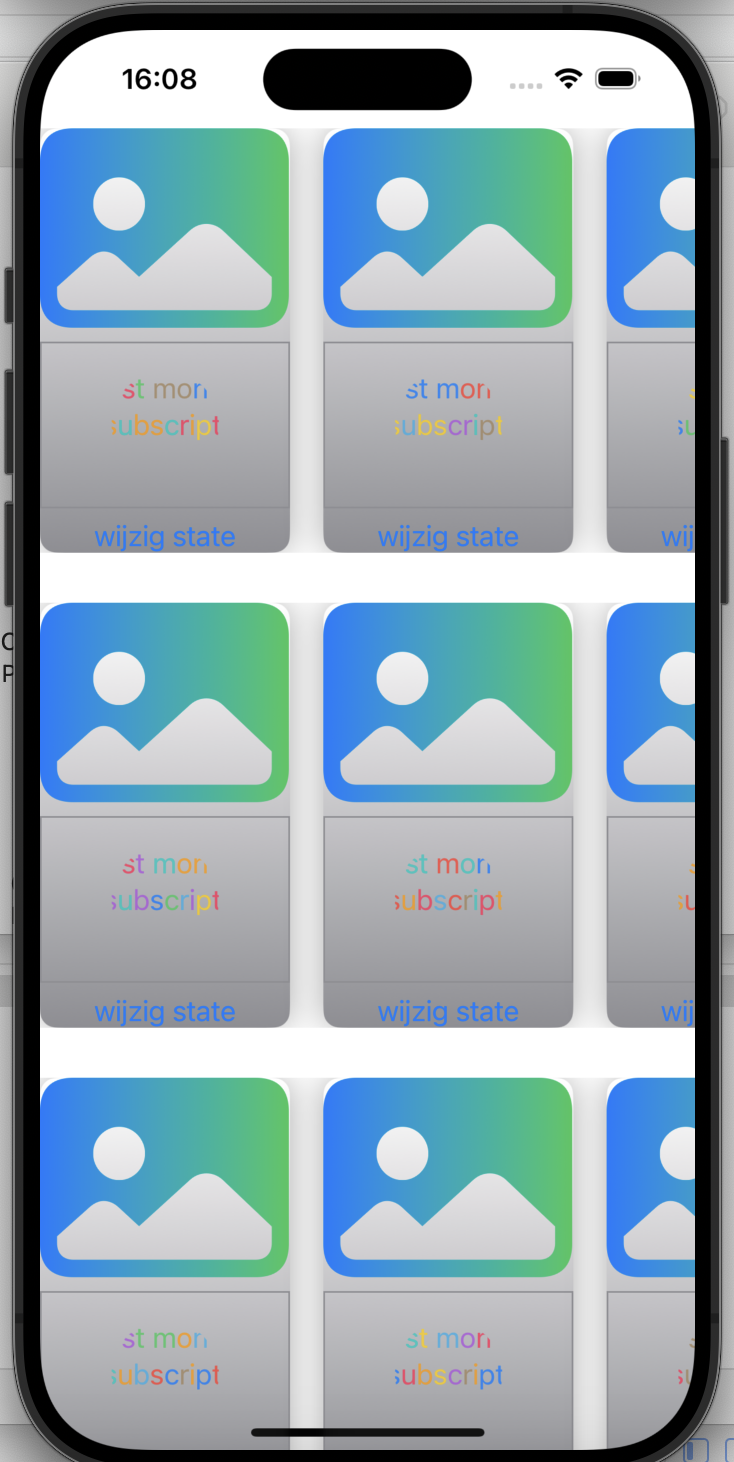
\includegraphics[width=0.4\textwidth]{testapplication} 
    \caption{testapplicatie}
    \label{fig:testapplication2}
\end{figure}
\begin{figure}[H]
    \centering
    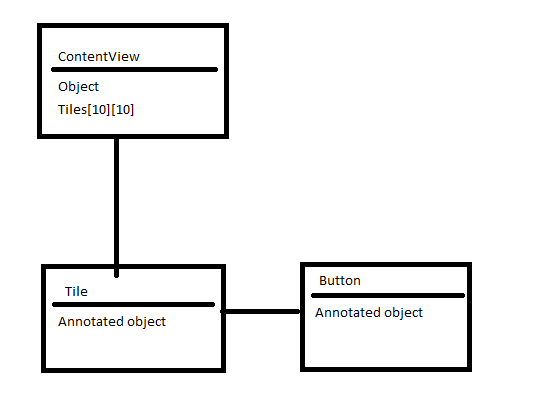
\includegraphics[width=0.4\textwidth]{bptest2_lazy/dataHierarchy} 
    \caption{testapplicatie data hierarchy}
    \label{fig:testapplicationHierarchy2}
\end{figure}

\subsection{Samengevat}
Onderstaande tabel bevat alle samengevatte resultaten uit deze test in 1 tabel gegoten. Uit deze tabel word er later in deze proef een conclusie getrokken.
\newpage
\begin{table}[H]
    \centering
    \begin{tabularx}{\textwidth}{|>{\raggedright\arraybackslash}m{5cm}|X|X|X|X|}
        \hline
        \textbf{Description} & \textbf{Binding} & \textbf{Observable} & \textbf{Environment Object} & \textbf{Observable Object} \\
        \hline
        \multicolumn{5}{|l|}{\textbf{Refresh count}} \\
        \hline
        ContentView refresh count & 10 & 1 & 0 & 0 \\
        \hline
        TileView refresh count & 90 & 99 & 90 & 90 \\
        \hline
        Button refresh count & N.V.T & N.V.T & N.V.T & N.V.T \\
        \hline
        Total refresh count & 100 & 100 & 90 & 90 \\
        \hline
        \multicolumn{5}{|l|}{\textbf{Refresh duration}} \\
        \hline
        ContentView total refresh duration & 269,46 \textmu s & 40,25 \textmu s & N.V.T & N.V.T \\
        \hline
        TileView total refresh duration & 1,93 ms & 2,08 ms & 1,85 ms & 2,1 ms \\
        \hline
        Button total refresh duration & N.V.T & N.V.T & N.V.T & N.V.T \\
        \hline
        Total duration & 2,30 ms & 2,12 ms & 1,85 ms & 2,1 ms \\
        \hline
        ContentView average refresh duration & 26,95 \textmu s & 40,25 \textmu s & N.V.T & N.V.T \\
        \hline
        TileView average refresh duration & 21,48 \textmu s & 20,97 \textmu s & 20,50 \textmu s & 23,33 \textmu s \\
        \hline
        Button average refresh duration & N.V.T & N.V.T & N.V.T & N.V.T \\
        \hline
        \multicolumn{5}{|l|}{\textbf{View property updates}} \\
        \hline
        ContentView property updates & 10 & 1 & 0 & 0 \\
        \hline
        TileView property updates & 90 & 9 & 90 & 90 \\
        \hline
        Button property updates & N.V.T & N.V.T & N.V.T & N.V.T \\
        \hline
        Total property updates & 100 & 10 & 90 & 90 \\
        \hline
        \multicolumn{5}{|l|}{\textbf{CPU usage}} \\
        \hline
        Total CPU usage time & 666 ms & 927 ms & 609 ms & 515 ms \\
        \hline
        Total CPU weight & 936,85 Mc & 463,30 Mc & 429,49 Mc & 862,21 Mc \\
        \hline
    \end{tabularx}
    \caption{Performance metrics comparison}
    \label{tab:performance_metrics2}
\end{table}


\section{Test4: Dataoverdracht naar meerdere subview's}
% Binding test 3
In deze sectie word de applicatie in de afbeelding hieronder gebruikt om de testen uit te voeren. Opgebouwd uit 1 VStack's die 10 HStack's bevat per HStack worden er 10 Tegels weergegeven. Elke tegel is zeer CPU heavy opgebouwd zodat de resultaten meer zichtbaar worden in de testen. Elke tile bevat ook een knop die een aanpassing van de testbare data gaat triggeren. In volgende afbeelding word de hierarchy afgebeeld. Voor elk type van dataoverdracht is er 10 keer op de button gedrukt voor het wijzigen van de view. Zo zijn de metingen tot stand gekomen. Alle ruwe resultaten die waargenomen zijn per datatype kan u terugvinden in bijlagen onder sectie Test4: Dataoverdracht naar meerdere subview'ss.
\begin{figure}[H]
    \centering
    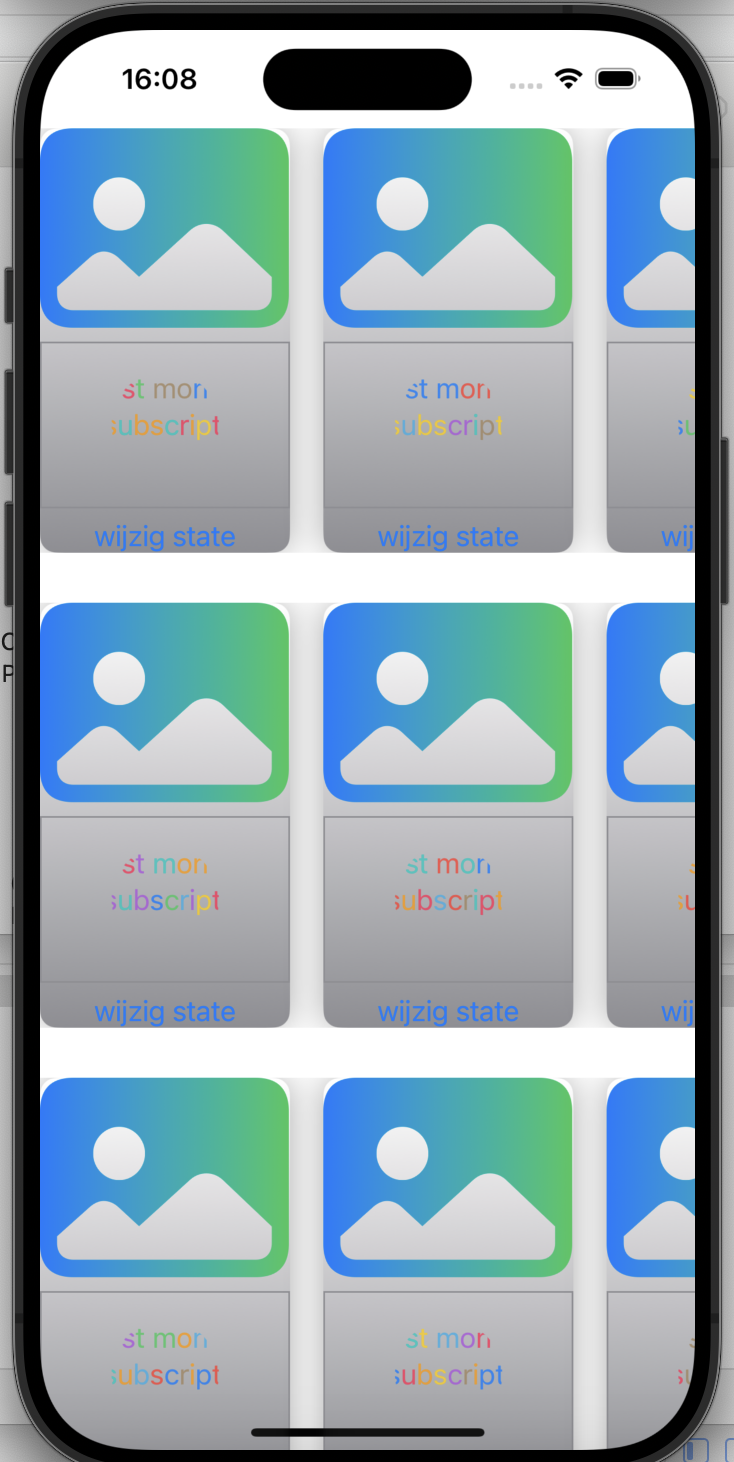
\includegraphics[width=0.4\textwidth]{testapplication} 
    \caption{testapplicatie}
    \label{fig:testapplication3}
\end{figure}
\begin{figure}[H]
    \centering
    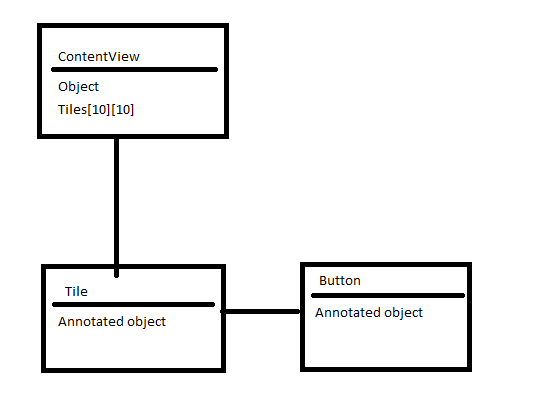
\includegraphics[width=0.4\textwidth]{bptest2_lazy/dataHierarchy} 
    \caption{testapplicatie data hierarchy}
    \label{fig:testapplicationHierarchy3}
\end{figure}


\subsection{Samengevat}
Onderstaande tabel bevat alle samengevatte resultaten uit deze test in 1 tabel gegoten. Uit deze tabel word er later in deze proef een conclusie getrokken.
\newpage
\begin{table}[H]
    \centering
    \begin{tabularx}{\textwidth}{|>{\raggedright\arraybackslash}m{5cm}|X|X|X|X|}
        \hline
        \textbf{Description} & \textbf{Binding} & \textbf{Observable} & \textbf{Environment Object} & \textbf{Observable Object} \\ \hline
        \textbf{Refresh count} & & & & \\ \hline
        ContentView refresh count & 10 & 0 & 0 & 0 \\ \hline
        TileView refresh count & 4410 & 4410 & 4410 & 4410 \\ \hline
        Button refresh count & N.V.T & N.V.T & N.V.T & N.V.T \\ \hline
        Total refresh count & 4420 & 4410 & 4410 & 4410 \\ \hline
        \textbf{Refresh duration} & & & & \\ \hline
        ContentView total refresh duration & 209,96 $\mu$s & N.V.T & N.V.T & N.V.T \\ \hline
        TileView total refresh duration & 30,15 ms & 23,24 ms & 24,49 ms & 24,33 ms \\ \hline
        Button total refresh duration & N.V.T & N.V.T & N.V.T & N.V.T \\ \hline
        Total duration & 30,36 ms & 23,24 ms & 24,49 ms & 24,33 ms \\ \hline
        ContentView average refresh duration & 6,87 $\mu$s & N.V.T & N.V.T & N.V.T \\ \hline
        TileView average refresh duration & 6,84 $\mu$s & 5,27 $\mu$s & 5,55 $\mu$s & 5,52 $\mu$s \\ \hline
        Button average refresh duration & N.V.T & N.V.T & N.V.T & N.V.T \\ \hline
        \textbf{View property updates} & & & & \\ \hline
        ContentView property updates & 10 & 0 & 0 & 0 \\ \hline
        TileView property updates & 4410 & 0 & 4410 & 4410 \\ \hline
        Button property updates & N.V.T & N.V.T & N.V.T & N.V.T \\ \hline
        Total property updates & 4420 & 0 & 4410 & 4410 \\ \hline
        \textbf{CPU usage} & & & & \\ \hline
        Total CPU usage time & 6,02 s & 4,8 s & 4,77 s & 4,81 s \\ \hline
        Total CPU weight & 12,93 Gc & 12,19 Gc & 12,10 Gc & 12,04 Gc \\ \hline
    \end{tabularx}
    \caption{Performance metrics}
\end{table}


\chapter{Resultaten}%
\label{ch:resultaten}
In dit hoofdstuk word er dieper in de onderzoeksresultaten van dit onderzoek gedelft. Alle resultaten zijn verkregen door de applicatie te testen via een Iphone 15 pro, IOS 17.4. Alle testen zijn ook systematisch 10 tot 100 keer overlopen voor een correcter resultaat. Van elke test word er nu een vergelijking gemaakt van de verschillende annotaties. Om zo tot een conclusie te komen.

\section{test2: het testen op een lege view met grote dataoverdracht}
Uit deze test blijkt dat de beste methode voor dataoverdracht binnen subviews op alle vlakken, behalve vernieuwingstijd, EnvironmentObject is. Als een snellere vernieuwingstijd vereist is, is ObservableObject een betere keuze, hoewel dit wel resulteert in een verdubbeling van de belasting op de CPU in vergelijking met andere methoden. De slechtste methode in deze test is de nieuwe Observable-macro, waarvan de totale vernieuwingstijd 4 tot 5 keer hoger ligt dan die van de andere methoden. 
\begin{table}[H]
    \centering
    
    \begin{tabularx}{\textwidth}{|>{\raggedright\arraybackslash}m{5cm}|X|X|X|X|}
        \hline
        \textbf{Description} & \textbf{Binding} & \textbf{Observable} & \textbf{Environment Object} & \textbf{Observable Object} \\ 
        \hline
        Total refresh count & \cellcolor{red!50}20 & \cellcolor{green!50}10 & \cellcolor{green!50}10 & \cellcolor{green!50}10 \\ 
        \hline
        Total duration & 214,58 \(\mu\)s & \cellcolor{red!50}1,82 ms & 214,58 \(\mu\)s & \cellcolor{green!50}125,63 \(\mu\)s \\ 
        \hline
        Total property updates & \cellcolor{red!50}20 & \cellcolor{red!50}20 & \cellcolor{green!50}10 & \cellcolor{green!50}10 \\ 
        \hline
        Total CPU usage time & \cellcolor{red!50}481 ms & \cellcolor{green!50}400 ms & \cellcolor{green!50}401 ms & 447 ms \\ 
        \hline
        Total CPU weight & \cellcolor{green!50}245,72 Mc & 294,88 Mc & \cellcolor{green!50}243,61 Mc & \cellcolor{red!50}653,23 Mc \\ 
        \hline
    \end{tabularx}
    \caption{Samengevatte resultaten van test2}
    \label{table:summary1}
\end{table}
\begin{itemize}
    \item \textcolor{green}{\textbf{Groen}}: Beste score
    \item \textcolor{red}{\textbf{Rood}}: Slechtste score
\end{itemize}

\section{Test3: Dataoverdracht naar meerdere subview's met lazyLists}
Uit deze test blijkt dat de beste methode voor dataoverdracht naar meerdere subview's met lazyLists op alle vlakken, behalve CPU usage time, EnvironmentObject is. Als een snellere CPU usage time vereist is, is ObservableObject een betere keuze, hoewel dit wel resulteert in een verdubbeling van de belasting op de CPU in vergelijking met andere methoden. De relatief slechtste methode in deze test is binding, deze scoort op vrijwel alle aspecten de slechtste score.  
\begin{table}[h!]
    \centering
     \begin{tabularx}{\textwidth}{|>{\raggedright\arraybackslash}m{5cm}|X|X|X|X|}
        \hline
        \textbf{Description} & \textbf{Binding} & \textbf{Observable} & \textbf{Environment Object} & \textbf{Observable Object} \\ 
        \hline
        Total refresh count & \cellcolor{red!50}100 & \cellcolor{red!50}100 & \cellcolor{green!50}90 & \cellcolor{green!50}90 \\ 
        \hline
        ContentView total refresh duration & 269,46 \(\mu\)s & 40,25 \(\mu\)s & N.V.T & N.V.T \\ 
        \hline
        TileView total refresh duration & 1,93 ms & 2,08 ms & 1,85 ms & 2,1 ms \\ 
        \hline
        Total duration & \cellcolor{red!50}2,30 ms & 2,12 ms & \cellcolor{green!50}1,85 ms & 2,1 ms \\ 
        \hline
        ContentView average refresh duration & 26,95 \(\mu\)s & 40,25 \(\mu\)s & N.V.T & N.V.T \\ 
        \hline
        TileView average refresh duration & 21,48 \(\mu\)s & 20,97 \(\mu\)s & 20,50 \(\mu\)s & 23,33 \(\mu\)s \\ 
        \hline
        View property updates & 10 & 1 & 0 & 0 \\ 
        \hline
        TileView property updates & 90 & 9 & 90 & 90 \\ 
        \hline
        Total property updates & \cellcolor{red!50}100 & \cellcolor{green!50}10 & 90 & 90 \\ 
        \hline
        Total CPU usage time & 666 ms & \cellcolor{red!50}927 ms & 609 ms & \cellcolor{green!50}515 ms \\ 
        \hline
        Total CPU weight & \cellcolor{red!50}936,85 Mc & 463,30 Mc & \cellcolor{green!50}429,49 Mc & 862,21 Mc \\ 
        \hline
    \end{tabularx}
    \caption{Samengevatte resultaten van test3}
    \label{table:summary2}
\end{table}

\begin{itemize}
    \item \textcolor{green}{\textbf{Groen}}: Beste score
    \item \textcolor{red}{\textbf{Rood}}: Slechtste score
\end{itemize}
\section{Test4: Dataoverdracht naar meerdere subview's}
Uit deze test blijkt dat de beste methode voor dataoverdracht naar meerdere subview's op alle vlakken, de nieuwe Observable macro is. EnvironmentObject, ObservableObject scoren bijna even goed als de observable macro. Binding daarintegen scoort op alle criteria het slechtste.
\begin{table}[H]
    \centering
    \begin{tabularx}{\textwidth}{|>{\raggedright\arraybackslash}m{5cm}|X|X|X|X|}
        \hline
        \textbf{Description} & \textbf{Binding} & \textbf{Observable} & \textbf{Environment Object} & \textbf{Observable Object} \\
        \hline
         ContentView refresh count & 10 & 0 & 0 & 0 \\
        \hline
         TileView refresh count & 4410 & 4410 & 4410 & 4410 \\
        \hline
        Total refresh count & \cellcolor{red!50} 4420 & \cellcolor{green!50}4410 & \cellcolor{green!50}4410 & \cellcolor{green!50}4410 \\
        \hline
         ContentView total refresh duration & 209.96 μs & N.V.T & N.V.T & N.V.T \\
        \hline
        TileView total refresh duration & 30.15 ms & 23.24 ms & 24.49 ms & 24.33 ms \\
        \hline
        Total duration &  \cellcolor{red!50}30.36 ms & \cellcolor{green!50}23.24 ms & \cellcolor{green!50}24.49 ms & \cellcolor{green!50}24.33 ms \\
        \hline
        ContentView average refresh duration & 6.87 μs & N.V.T & N.V.T & N.V.T \\
        \hline
        TileView average refresh duration & 6.84 μs & 5.27 μs & 5.55 μs & 5.52 μs \\
        \hline
         ContentView property updates & 10 & 0 & 0 & 0 \\
        \hline
        TileView property updates & 4410 & 0 & 4410 & 4410 \\
        \hline
        Total property updates & \cellcolor{red!50} 4420 & \cellcolor{green!50}0 & 4410 & 4410 \\
        \hline
        Total CPU usage time & \cellcolor{red!50} 6.02 s & \cellcolor{green!50}4.8 s & \cellcolor{green!50}4.77 s & \cellcolor{green!50}4.81 s \\
        \hline
        Total CPU weight & \cellcolor{red!50} 12.93 Gc & \cellcolor{green!50}12.19 Gc & \cellcolor{green!50}12.10 Gc & \cellcolor{green!50}12.04 Gc \\
        \hline
    \end{tabularx}
    \caption{Samengevatte resultaten van test4}
    \label{table:summary3}
\end{table}

%%=============================================================================
%% Conclusie
%%=============================================================================

\chapter{Conclusie}%
\label{ch:conclusie}

% TODO: Trek een duidelijke conclusie, in de vorm van een antwoord op de
% onderzoeksvra(a)g(en). Wat was jouw bijdrage aan het onderzoeksdomein en
% hoe biedt dit meerwaarde aan het vakgebied/doelgroep? 
% Reflecteer kritisch over het resultaat. In Engelse teksten wordt deze sectie
% ``Discussion'' genoemd. Had je deze uitkomst verwacht? Zijn er zaken die nog
% niet duidelijk zijn?
% Heeft het onderzoek geleid tot nieuwe vragen die uitnodigen tot verder 
%onderzoek?


\section{Analyse van Gegevensoverdrachtmethoden in SwiftUI Views}
Op basis van de voorgaande gegevens kunnen we de invloed van diverse methoden van gegevensoverdracht naar SwiftUI views op de performance, renderingfrequentie en levenscyclussen van bindings als volgt analyseren:

\subsection{Performance}
De performance wordt gemeten aan de hand van de totale CPU-gebruikstijd en de totale CPU-weight:
\begin{itemize}
    \item \textit{EnvironmentObject} en \textit{ObservableObject} scoren over het algemeen goed qua CPU-gebruik, waarbij ObservableObject iets meer CPU-belasting veroorzaakt.
    \item \textit{Binding} presteert consistent slecht qua CPU-gebruik, vooral in complexe scenario's met meerdere subviews.
    \item \textit{Observable} presteert slechter dan andere methoden qua totale vernieuwingstijd in sommige tests.
\end{itemize}

\subsection{Renderingfrequentie}
De renderingfrequentie wordt gemeten aan de hand van het totaal aantal vernieuwingen en de totale duur van vernieuwingen:
\begin{itemize}
    \item \textit{EnvironmentObject} biedt een balans tussen frequentie en duur van vernieuwingen en is meestal efficiënter in de totale duur van vernieuwingen.
    \item \textit{ObservableObject} heeft de kortste totale vernieuwingstijd, wat het geschikt maakt voor scenario's waar snelle vernieuwingen cruciaal zijn.
    \item \textit{Observable} heeft een hogere totale vernieuwingstijd, wat kan leiden tot tragere updates.
\end{itemize}

\subsection{Property updates van Bindings}
De property updates van bindings beïnvloedt hoe vaak gegevens bijgewerkt worden:
\begin{itemize}
    \item \textit{Observable}: Deze methode vereist minder frequente updates, dit heeft te maken met dat observable gemaakt is voor onnodige view redraws, dit zorgt ook voor een lagere CPU belasting.
    \item \textit{Binding}: Deze methode vereist frequente updates, wat kan leiden tot hogere CPU-belasting en langere vernieuwingstijden.
    \item \textit{EnvironmentObject en ObservableObject}: Deze bieden een meer gestructureerde en efficiënte manier om gegevens over te dragen, wat leidt tot minder frequente updates.
\end{itemize}

\newpage
\section{Vergelijking van "Observable" met Andere Methoden}

De "Observable" macro is een nieuwere methode van Apple die bedoeld is om andere ``observable''-methoden voor gegevensoverdracht in SwiftUI te vervangen. Hieronder volgt een gedetailleerde vergelijking van "Observable" met \textit{Binding}, \textit{EnvironmentObject} en \textit{ObservableObject} op basis van performance, renderingfrequentie en levenscyclussen van bindings.

\subsection{Performance}
De performance wordt gemeten aan de hand van de totale CPU-gebruikstijd en het totale CPU-gewicht:
\begin{itemize}
    \item \textit{Observable} scoort beter dan \textit{Binding}, maar slechter dan \textit{EnvironmentObject} en \textit{ObservableObject} qua CPU-gebruik. 
    \item \textit{Observable} heeft een CPU-gebruikstijd van 400 ms in Test2 en 927 ms in Test3, wat beter is dan Binding maar slechter dan de andere methoden.
    \item De totale CPU-gewicht voor \textit{Observable} is 294,88 Mc in Test2 en 463,30 Mc in Test3, wat betekent dat het een zwaardere belasting heeft dan \textit{EnvironmentObject}, maar minder dan \textit{Binding} en \textit{ObservableObject}.
\end{itemize}

\subsection{Renderingfrequentie}
De renderingfrequentie wordt gemeten aan de hand van het totaal aantal vernieuwingen en de totale duur van vernieuwingen:
\begin{itemize}
    \item \textit{Observable} heeft een hogere totale vernieuwingstijd in Test2 (1,82 ms) en een gematigde score in Test3 (2,12 ms) vergeleken met andere methoden.
    \item De totale vernieuwingstijd is slechter dan \textit{EnvironmentObject} en \textit{ObservableObject}, maar beter dan \textit{Binding}.
    \item De totale vernieuwingen in Test2 en Test3 laten zien dat \textit{Observable} efficiënter is dan \textit{Binding} maar minder efficiënt dan \textit{EnvironmentObject} en \textit{ObservableObject}.
\end{itemize}


De "Observable" macro van Apple is een moderne methode voor gegevensoverdracht in SwiftUI, die is ontworpen om oudere methoden zoals \textit{Binding}, \textit{EnvironmentObject}, en \textit{ObservableObject} te vervangen of aan te vullen. Op basis van de uitgevoerde tests en analyse kunnen we de volgende conclusies trekken:

\subsection{Voordelen van ``Observable''}
\begin{itemize}
    \item \textit{Verbeterde Performance}: De ``Observable'' macro presteert beter dan \textit{Binding} in termen van CPU-gebruik en vernieuwingstijden. Dit maakt het een efficiëntere keuze voor complexere UI's waar prestaties kritisch zijn.
    \item \textit{Efficiëntere Renderingfrequentie}: De totale vernieuwingstijd voor "Observable" is lager dan die van \textit{Binding}, wat resulteert in vloeiendere en snellere UI-updates.
    \item \textit{Lagere Frequentie van Updates}: "Observable" vereist minder frequente updates dan \textit{Binding}, wat de levensduur van de binding verlengt en de CPU-belasting vermindert.
\end{itemize}

\subsection{Conclusie}
De "Observable" macro is een aanzienlijke verbetering ten opzichte van \textit{Binding} en biedt een modernere en efficiëntere aanpak voor gegevensoverdracht in SwiftUI. Hoewel \textit{EnvironmentObject} en \textit{ObservableObject} vaak betere prestaties leveren, is ``Observable'' een aantrekkelijke keuze voor ontwikkelaars die een balans zoeken tussen gebruiksgemak en efficiëntie. Het gebruik van "Observable" kan leiden tot betere prestaties en een responsievere gebruikersinterface in veel scenario's, waardoor het een waardevolle toevoeging is aan de toolkit van elke SwiftUI-ontwikkelaar.


\newpage
\section{Conclusie en Aanbevelingen}
\begin{itemize}
    \item \textbf{EnvironmentObject} is geschikt voor scenario's waar een balans tussen prestaties en vernieuwingstijden belangrijk is. Het biedt efficiënte gegevensoverdracht met een lage CPU-belasting.
    \item \textbf{ObservableObject} is ideaal wanneer snelle vernieuwingstijden cruciaal zijn, ondanks de hogere CPU-belasting.
    \item \textbf{Binding} moet vermeden worden in complexe UI's met meerdere subviews vanwege de hoge CPU-belasting en frequente updates.
    \item \textbf{Observable} is minder efficiënt in termen van vernieuwingstijden en moet alleen worden gebruikt wanneer specifieke voordelen van deze methode nodig zijn.
\end{itemize}

\subsection{Gebruik van Bevindingen}
Bij het ontwerpen van efficiënte gebruikersinterfaces kunnen deze bevindingen als volgt worden benut:
\begin{itemize}
    \item Kies \textbf{EnvironmentObject} voor algemene doeleinden en grotere applicaties waar meerdere subviews gegevens moeten delen.
    \item Gebruik \textbf{ObservableObject} in scenario's waar snelle responstijden cruciaal zijn, zoals bij real-time data updates.
    \item Vermijd \textbf{Binding} en \textit{Observable} in complexe of prestatiekritieke delen van de applicatie om inefficiënties te voorkomen.
\end{itemize}

Door deze methoden strategisch te kiezen op basis van de hierboven beschreven performance en efficiëntie kunnen ontwikkelaars goed presterende en responsieve gebruikersinterfaces in SwiftUI ontwerpen.





%---------- Bijlagen -----------------------------------------------------------

\appendix

\chapter{Onderzoeksvoorstel}

Het onderwerp van deze bachelorproef is gebaseerd op een onderzoeksvoorstel dat vooraf werd beoordeeld door de promotor. Dat voorstel is opgenomen in deze bijlage.

%% TODO: 
\section*{Samenvatting}
% Kopieer en plak hier de samenvatting (abstract) van je onderzoeksvoorstel.

Dit bachelorproefvoorstel beoogt een diepgaande analyse van diverse methoden voor gegevensoverdracht naar
SwiftUI-views, met een focus op de impact op performance, rendering en lifecycles. Het onderzoek zal een uitgebreide
lijst van dataoverdrachtsmethoden omvatten, waarbij de nadruk ligt op het identificeren van verschillen
in rendercyclussen. We zullen de frequentie van view-rendering onderzoeken, de algehele prestaties evalueren
en de levenscycli van deze bindings analyseren. Door deze vergelijkende studie streven we ernaar om inzichten
te brengen in de meest efficiënte methoden voor gegevensoverdracht in SwiftUI, waardoor ontwikkelaars beter
geïnformeerde beslissingen kunnen nemen bij het ontwerpen van responsieve en performante gebruikersinterfaces.

% Verwijzing naar het bestand met de inhoud van het onderzoeksvoorstel
%---------- Inleiding ---------------------------------------------------------

\section{Introductie}%
\label{sec:introductie}

In deze bachelorproef word een grondige verkenning van de rendercyclussen in SwiftUI gedaan, met een specifieke focus op de impact ervan op prestaties, rendering en de levenscyclus van bindings. SwiftUI, een innovatief framework voor het bouwen van gebruikersinterfaces in Swift, heeft de ontwikkeling van iOS-applicaties getransformeerd door de introductie van declaratieve syntax en reactieve programmeerprincipes. In deze bachelorproef willen we de verschillende methoden voor gegevensoverdracht naar SwiftUI-views identificeren en analyseren, met als ultiem doel ontwikkelaars inzicht te verschaffen in de meest efficiënte benaderingen voor het bereiken van de beste UI-prestaties.

\subsection{Doelgroep}
Deze studie richt zich op softwareontwikkelaars, met een specifieke interesse in iOS-applicatie ontwikkeling en SwiftUI. Het biedt een diepgaand inzicht in de keuzemogelijkheden voor data-overdracht en de gevolgen ervan op de algehele gebruikersinterface.

\subsection{Probleemstelling}
De diversiteit aan beschikbare methoden voor het doorgeven van gegevens in SwiftUI roept vragen op over de optimale keuze voor specifieke gebruiksscenario's. Het gebrek aan diepgaande vergelijkende studies maakt het voor ontwikkelaars moeilijk om beslissingen te nemen bij het ontwerpen van efficiënte gebruikersinterfaces.

\subsection{Centrale onderzoeksvraag}
In hoeverre beïnvloeden diverse methoden van gegevensoverdracht naar SwiftUI views de performance, renderingfrequentie en levenscyclussen van bindings, en hoe kunnen deze bevindingen worden benut om weloverwogen keuzes te maken bij het ontwerpen van efficiënte gebruikersinterfaces?

\subsection{Onderzoeksdoelstelling}
Deze bachelorproef beoogt een diepgaand begrip van de rendercyclussen in SwiftUI en streeft ernaar om ontwikkelaars te voorzien van concrete richtlijnen voor het optimaliseren van de prestaties en rendering van hun iOS-applicaties. Door een vergelijkende analyse van de verschillende dataoverdrachtsmethoden wordt beoogd heldere aanbevelingen te formuleren voor effectieve UI-implementaties in SwiftUI.


%---------- Stand van zaken ---------------------------------------------------

\section{Literatuurstudie}%
\label{sec:state-of-the-art}

Uit al de volgende bronnen kunnen we informatie halen omtrent verschillende manieren van data doorgeven in SwiftUI. Zo zijn er deze 6 Veelgebruikte methoden:
\newline\textbf{@State:}
\begin{itemize}
    \item {Lokale en eenvoudige gegevensopslag die het gedrag van een view beïnvloeden.}
    \item {Wordt meestal gebruikt voor primitieve gegevenstypes zoals integers, strings en boole-\newline ans.}
\end{itemize}
\textbf{@Binding:}
\begin{itemize}
    \item {Het doorgeven van gegevens tussen de ouder-view en de onderliggende view.}
    \item {De waarde wordt doorgegeven als een binding, waardoor de onderliggende view de waarde kan wijzigen.}
\end{itemize}
\textbf{@ObservedObject:}
\begin{itemize}
    \item {Het doorgeven van gegevens die door een externe klasse worden beheerd en waarmee de view wordt geïnformeerd over wijzigingen.}
    \item {Vereist het gebruik van een ObservableObject klasse.}
\end{itemize}
\textbf{@StateObject:}
\begin{itemize}
    \item {Vergelijkbaar met @ObservedObject, maar met een levenscyclus die is gebonden aan de view.}
    \item {Wordt geïnitialiseerd en beheerd door de view en kan worden gebruikt voor het bijhouden van de status van de view.}
\end{itemize}
\textbf{@Observable:}
\begin{itemize}
    \item {Een vervanging van vele oude methodes zoals State en Environment}
    \item {Apple claimed dat deze nieuwe macro performanter is}
\end{itemize}




De volgende macro's zijn niet vergelijkbaar met de andere omdat deze een specifiek doel hebben maar zijn nog steeds de moeite om te vermelden:
\newline\textbf{@EnvironmentObject:}
\begin{itemize}
    \item {Het doorgeven van gegevens die door een externe klasse worden beheerd, toegankelijk voor de hele app zonder expliciete doorgifte.}
    \item {Vereist het gebruik van een ObservableObject-klasse en wordt vaak gebruikt voor gedeelde gegevens zoals gebruikersauthenticatie.}
\end{itemize}
\textbf{@Binding in init:}
\begin{itemize}
    \item {Het initialiseren van een binding tijdens de init-fase van een view.}
    \item {Maakt het mogelijk om een binding te maken en door te geven bij de creatie van de view.}
\end{itemize}

% Dit is vloeiende tekst
% Uit enkele relevante studies kunnen we concluderen dat er veel vraag en verwarring is rond de correcte manier van data doorgeven aan SwiftUI views. Verschillende bronnen benadrukken dit thema en bieden waardevolle inzichten. Het artikel "Passing Data to SwiftUI Views"~\autocite{SwiftDevJournal} identificeert expliciet drie methoden voor gegevensoverdracht aan views, wat cruciale informatie verschaft voor een dieper begrip van dit onderwerp. Bovendien onthult de studie "Deep Inside Views, State and Performance in SwiftUI"~\autocite{Long2020} dat veel bedrijven en ontwikkelaars nog steeds vasthouden aan de denkwijze van UIKit, wat potentieel verwarrend kan zijn bij het doorgeven van gegevens naar views in SwiftUI. Deze bevindingen benadrukken het belang van een helder begrip van de verschillen tussen UIKit en SwiftUI views. Binnen het kader van prestatieoptimalisatie, zoals besproken in "SwiftUI Performance Tuning: Tips and Tricks"~\autocite{Amisha2022}, wordt aanbevolen om de annotaties @Binding en @State te gebruiken voor efficiënte gegevensoverdracht, aangezien deze methoden een betere prestatie laten zien in vergelijking met @ObservedObject en @EnvironmentObject.

\textbf{Passing Data to SwiftUI Views~\autocite{SwiftDevJournal}}

In dit artikel worden waardevolle inzichten gepresenteerd met betrekking tot diverse benaderingen voor het doorgeven van gegevens naar SwiftUI-views. Het artikel identificeert expliciet drie methoden voor gegevensoverdracht aan views en biedt daarmee cruciale informatie voor ons begrip van dit onderwerp.

\textbf{Deep Inside Views, State and Performance in SwiftUI~\autocite{Long2020}}

Deze bron onthult dat veel bedrijven en softwareontwikkelaars nog steeds vasthouden aan de denkwijze van UIKit in plaats van de nieuwe benadering van SwiftUI-views. Het is van belang te benadrukken dat UIKit en SwiftUI views twee verschillende concepten zijn. Deze neiging om vast te houden aan de oudere UIKit-mentaliteit kan potentiële verwarring veroorzaken bij het doorgeven van gegevens naar views in SwiftUI.

\textbf{SwiftUI Performance Tuning: Tips and Tricks\newline ~\autocite{Amisha2022}}

Uit deze bron blijkt dat het gebruik van de annotaties @Binding en @State voor het doorgeven van gegevens efficiënter is dan het gebruik van @ObservedObject en @EnvironmentObject.


\textbf{Pro iPhone Development with SwiftUI~\autocite{WangWallace2022PIDw}}

Uit dit onderzoek kunnen we halen dat State variabelen handig zijn voor het opslaan van afzonderlijke data blocks zoals integers (Int), decimale getallen (Double of Float), of tekst (String). Bindingsvariabelen zijn nuttig voor het aanpassen van Staatsvariabelen vanuit een andere structuur dan de structuur die de State variabele heeft gedefinieerd.

\textbf{Asynchronous Programming with SwiftUI and Combine: Functional Programming to Build UIs on Apple Platforms~\autocite{friese2023state}}

Uit dit boek kunnen we ook halen dat een @StateObject, @ObservedObject, of @EnvironmentObject, dus een ObservableObject gererenderd worden wanneer SwiftUi een verandering registreert binnen het State model. Dit houd in dat SwiftUI de actuele data in sync houd met de data die weergegeven word in de View. Ook kunnen we nuttige info vergaren uit dit boek over @StateObject. Ze beweren dat SwiftUi de lifecycle van het onderliggend object beheerd en zo er ook voor zou zorgen dat het maar 1 keer aangemaakt zou worden, Zelfs als SwiftUI de hele View opnieuw zou moeten maken. In tegenstelling tot @StateObject wordt @ObservedObject elke keer herbouwt nadat een SwiftUi View wordt herbouwd.

Uit dit artikel kunnen we ook leren dat @EnvironmentObject geen veilige manier is van dataoverdracht omdat deze niet controleert of er wel een ObservableObject word geïnjecteerd. Hierdoor kan de applicatie onverwachts crashen.



% Voor literatuurverwijzingen zijn er twee belangrijke commando's:
% \autocite{KEY} => (Auteur, jaartal) Gebruik dit als de naam van de auteur
%   geen onderdeel is van de zin.
% \textcite{KEY} => Auteur (jaartal)  Gebruik dit als de auteursnaam wel een
%   functie heeft in de zin (bv. ``Uit onderzoek door Doll & Hill (1954) bleek
%   ...'')



%---------- Methodologie ------------------------------------------------------
\section{Methodologie}%
\label{sec:methodologie}

\subsection{Onderzoekstechniek}
Dit onderzoek zal hoofdzakelijk gebruikmaken van een vergelijkende studie om de impact van verschillende methoden voor gegevensoverdracht naar SwiftUI views te analyseren. De primaire focus ligt op het vergelijken van de prestaties, renderingfrequentie en levenscycli van bindings bij het toepassen van verschillende benaderingen. De vergelijkende studie omvat het oplijsten van alle verschillende manieren om data door te geven aan SwiftUI views en langs elkaar zetten wat ieder zijn impact op performance is, hoeveel keer views gererendered  worden en wat de lifecycles van deze bindings zijn. 

\subsection{Tools}
\textbf{Xcode en SwiftUI Framework}

De ontwikkelingsomgeving Xcode, met het SwiftUI framework, zal worden gebruikt om praktische implementaties uit te voeren en de impact van verschillende dataoverdrachtsmethoden te meten.

\textbf{XCode Profiler}

Met dit instrument kunnen we performantie gaan tracken door middel van CPU usage en memory problems.

\textbf{XCTest framework}

Dit framework zorgt ervoor dat we performantie kunnen waarnemen in swiftUI.

\textbf{Google en Apple Developer Website}

Deze applicaties gaan we gebruiken om info te vergaren over SwiftUI en de werking van Swift.


\subsection{Tijdschatting}
De totale geschate tijd die nodig is zijn 15 weken waarbij ruimte is voor mogelijke aanpassingen afhankelijk van de specifieke behoeften van elke fase.

\textbf{Voorstel}
\begin{itemize}
    \item {2 Weken}
    \item {Voorstel uitschrijven in een LaTeX document}
    \item {Opzetten van github repo}
\end{itemize}

\textbf{Implementatie en metingen}
\begin{itemize}
    \item {8 Weken}
    \item {Gedocumenteerde implementatie van de onderzoeksopdracht}
    \item {Meetresultaten waarnemen van presentaties en rendering}
\end{itemize}

\textbf{Vergelijkende analyse}
\begin{itemize}
    \item {1 Week}
    \item {Analyse van de resultaten en vergelijken}
\end{itemize}

\textbf{Schrijven thesis}
\begin{itemize}
    \item {4 Weken}
    \item {Voltooide thesis met inbegrip van introductie, literatuurstudie, methodologie, resultaten, discussie, conclusies}
\end{itemize}



%---------- Verwachte resultaten ----------------------------------------------
\section{Verwacht resultaat, conclusie}
\label{sec:verwachte_resultaten}


\subsection{Verwacht resultaat}
We verwachten uit de vergelijkende studie een duidelijk inzicht te verkrijgen in de impact van verschillende methoden voor gegevensoverdracht naar SwiftUI views op prestaties, renderingfrequentie en levenscycli van bindings. De metingen zullen waarschijnlijk resulteren in kwantificeerbare gegevens die de efficiëntie van de @Binding, @State, @ObservedObject en @EnvironmentObject in verschillende scenario's illustreren.

\subsection{Conclusie}
We verwachten dat de @Binding en @State het best zullen uitkomen wat betreft prestaties en renderingfrequentie, terwijl @ObservedObject en @EnvironmentObject mogelijk meer resources vereisen. De levenscyclusgrafiek van bindings zal waarschijnlijk aangeven dat @Binding en @State bindings een meer voorspelbare levensduur hebben in vergelijking met @ObservedObject en @EnvironmentObject.

\subsection{Meerwaarde doelgroep}
De doelgroep, bestaande uit SwiftUI ontwikkelaars en IOS applicatie ontwikkelaars, zal profiteren van concrete inzichten in welke gegevensoverdrachtsmethoden de voorkeur verdienen in verschillende scenario's. Door de resultaten van dit onderzoek kunnen zij goede keuzes maken bij het ontwerpen van efficiënte gebruikersinterfaces in SwiftUI. De meerwaarde van deze bachelorproef ligt in het bieden van praktische richtlijnen die direct toepasbaar zijn in de dagelijkse praktijk van iOS applicatieontwikkeling, en zo bijdragen aan de optimalisatie van SwiftUI gebaseerde projecten.




%%---------- Andere bijlagen --------------------------------------------------
% TODO: Voeg hier eventuele andere bijlagen toe. Bv. als je deze BP voor de
% tweede keer indient, een overzicht van de verbeteringen t.o.v. het origineel.
%\input{...}

%%---------- Backmatter, referentielijst ---------------------------------------

\backmatter{}

\setlength\bibitemsep{2pt} %% Add Some space between the bibliograpy entries
\printbibliography[heading=bibintoc]

\end{document}
